% Options for packages loaded elsewhere
% Options for packages loaded elsewhere
\PassOptionsToPackage{unicode}{hyperref}
\PassOptionsToPackage{hyphens}{url}
\PassOptionsToPackage{dvipsnames,svgnames,x11names}{xcolor}
%
\documentclass[
  letterpaper,
  DIV=11,
  numbers=noendperiod]{scrartcl}
\usepackage{xcolor}
\usepackage[lmargin=1.5cm,rmargin=1.5cm,tmargin=1.5cm,bmargin=1.5cm]{geometry}
\usepackage{amsmath,amssymb}
\setcounter{secnumdepth}{5}
\usepackage{iftex}
\ifPDFTeX
  \usepackage[T1]{fontenc}
  \usepackage[utf8]{inputenc}
  \usepackage{textcomp} % provide euro and other symbols
\else % if luatex or xetex
  \usepackage{unicode-math} % this also loads fontspec
  \defaultfontfeatures{Scale=MatchLowercase}
  \defaultfontfeatures[\rmfamily]{Ligatures=TeX,Scale=1}
\fi
\usepackage{lmodern}
\ifPDFTeX\else
  % xetex/luatex font selection
\fi
% Use upquote if available, for straight quotes in verbatim environments
\IfFileExists{upquote.sty}{\usepackage{upquote}}{}
\IfFileExists{microtype.sty}{% use microtype if available
  \usepackage[]{microtype}
  \UseMicrotypeSet[protrusion]{basicmath} % disable protrusion for tt fonts
}{}
\makeatletter
\@ifundefined{KOMAClassName}{% if non-KOMA class
  \IfFileExists{parskip.sty}{%
    \usepackage{parskip}
  }{% else
    \setlength{\parindent}{0pt}
    \setlength{\parskip}{6pt plus 2pt minus 1pt}}
}{% if KOMA class
  \KOMAoptions{parskip=half}}
\makeatother
% Make \paragraph and \subparagraph free-standing
\makeatletter
\ifx\paragraph\undefined\else
  \let\oldparagraph\paragraph
  \renewcommand{\paragraph}{
    \@ifstar
      \xxxParagraphStar
      \xxxParagraphNoStar
  }
  \newcommand{\xxxParagraphStar}[1]{\oldparagraph*{#1}\mbox{}}
  \newcommand{\xxxParagraphNoStar}[1]{\oldparagraph{#1}\mbox{}}
\fi
\ifx\subparagraph\undefined\else
  \let\oldsubparagraph\subparagraph
  \renewcommand{\subparagraph}{
    \@ifstar
      \xxxSubParagraphStar
      \xxxSubParagraphNoStar
  }
  \newcommand{\xxxSubParagraphStar}[1]{\oldsubparagraph*{#1}\mbox{}}
  \newcommand{\xxxSubParagraphNoStar}[1]{\oldsubparagraph{#1}\mbox{}}
\fi
\makeatother


\usepackage{longtable,booktabs,array}
\newcounter{none} % for unnumbered tables
\usepackage{calc} % for calculating minipage widths
% Correct order of tables after \paragraph or \subparagraph
\usepackage{etoolbox}
\makeatletter
\patchcmd\longtable{\par}{\if@noskipsec\mbox{}\fi\par}{}{}
\makeatother
% Allow footnotes in longtable head/foot
\IfFileExists{footnotehyper.sty}{\usepackage{footnotehyper}}{\usepackage{footnote}}
\makesavenoteenv{longtable}
\usepackage{graphicx}
\makeatletter
\newsavebox\pandoc@box
\newcommand*\pandocbounded[1]{% scales image to fit in text height/width
  \sbox\pandoc@box{#1}%
  \Gscale@div\@tempa{\textheight}{\dimexpr\ht\pandoc@box+\dp\pandoc@box\relax}%
  \Gscale@div\@tempb{\linewidth}{\wd\pandoc@box}%
  \ifdim\@tempb\p@<\@tempa\p@\let\@tempa\@tempb\fi% select the smaller of both
  \ifdim\@tempa\p@<\p@\scalebox{\@tempa}{\usebox\pandoc@box}%
  \else\usebox{\pandoc@box}%
  \fi%
}
% Set default figure placement to htbp
\def\fps@figure{htbp}
\makeatother





\setlength{\emergencystretch}{3em} % prevent overfull lines

\providecommand{\tightlist}{%
  \setlength{\itemsep}{0pt}\setlength{\parskip}{0pt}}



 


\usepackage{array}
\providecommand{\huxb}[2]{\arrayrulecolor[RGB]{#1}\global\arrayrulewidth=#2pt}
\providecommand{\huxvb}[2]{\color[RGB]{#1}\vrule width #2pt}
\providecommand{\huxtpad}[1]{\rule{0pt}{#1}}
\providecommand{\huxbpad}[1]{\rule[-#1]{0pt}{#1}}
\usepackage{caption}
\usepackage{graphicx}
\usepackage{siunitx}
\usepackage[normalem]{ulem}
\usepackage{colortbl}
\usepackage{multirow}
\usepackage{hhline}
\usepackage{calc}
\usepackage{tabularx}
\usepackage{longtable}
\usepackage{threeparttable}
\usepackage{threeparttablex}
\usepackage{wrapfig}
\usepackage{adjustbox}
\usepackage{hyperref}
\usepackage{cancel}
\KOMAoption{captions}{tableheading}
\makeatletter
\@ifpackageloaded{caption}{}{\usepackage{caption}}
\AtBeginDocument{%
\ifdefined\contentsname
  \renewcommand*\contentsname{Table of contents}
\else
  \newcommand\contentsname{Table of contents}
\fi
\ifdefined\listfigurename
  \renewcommand*\listfigurename{List of Figures}
\else
  \newcommand\listfigurename{List of Figures}
\fi
\ifdefined\listtablename
  \renewcommand*\listtablename{List of Tables}
\else
  \newcommand\listtablename{List of Tables}
\fi
\ifdefined\figurename
  \renewcommand*\figurename{Figure}
\else
  \newcommand\figurename{Figure}
\fi
\ifdefined\tablename
  \renewcommand*\tablename{Table}
\else
  \newcommand\tablename{Table}
\fi
}
\@ifpackageloaded{float}{}{\usepackage{float}}
\floatstyle{ruled}
\@ifundefined{c@chapter}{\newfloat{codelisting}{h}{lop}}{\newfloat{codelisting}{h}{lop}[chapter]}
\floatname{codelisting}{Listing}
\newcommand*\listoflistings{\listof{codelisting}{List of Listings}}
\makeatother
\makeatletter
\makeatother
\makeatletter
\@ifpackageloaded{caption}{}{\usepackage{caption}}
\@ifpackageloaded{subcaption}{}{\usepackage{subcaption}}
\makeatother
\usepackage{bookmark}
\IfFileExists{xurl.sty}{\usepackage{xurl}}{} % add URL line breaks if available
\urlstyle{same}
% fallback for those not using the hyperref driver hyperxmp:
\makeatletter
\@ifundefined{xmpquote}{\newcommand{\xmpquote}[1]{#1}}{}
\makeatother
\hypersetup{
  pdftitle={Measurement of Policy Outcomes: Homework 3},
  pdfauthor={BELTRAN GONZALEZ Luis Enrique},
  colorlinks=true,
  linkcolor={blue},
  filecolor={Maroon},
  citecolor={Blue},
  urlcolor={Blue},
  pdfcreator={LaTeX via pandoc}}


\title{Measurement of Policy Outcomes: Homework 3}
\usepackage{etoolbox}
\makeatletter
\providecommand{\subtitle}[1]{% add subtitle to \maketitle
  \apptocmd{\@title}{\par {\large #1 \par}}{}{}
}
\makeatother
\subtitle{Applied Analysis of Living Standards and Economic Inequality
in Côte d'Ivoire}
\author{BELTRAN GONZALEZ Luis Enrique}
\date{2026-11-24}
\begin{document}
\maketitle


\section{Sampling and Outliers}\label{sampling-and-outliers}

\textbf{1.a} \textbf{Highly unequal samples are difficult to measure and
could be underrepresented.} Groups in rural settings or difficult survey
conditions are likely underrepresented because the costs and efforts to
reach them are high. For example, in Mexico, indigenous people face high
inequality and often live in hard-to-reach rural areas, have lower
literacy levels, and do not speak Spanish, making them difficult to
measure and underrepresented in surveys. \textbf{Low sample number and
high variance.} By definition, inequality implies measuring samples far
from the population mean (e.g., households with extreme low income).
Measuring the left or right tail requires sampling from a small group,
which limits the number of potential samples and increases the variance
and confidence intervals for that group. \textbf{People might lie or
misreport their income or consumption.} Respondents may misreport income
or consumption because they fear being taxed, feel ashamed of low
income, or struggle to recall their consumption accurately.

\textbf{1.b} It changes the inequality threshold and might leave out
people under inequality conditions. Outliers affect the estimates used
to identify people facing inequality conditions. For example, under the
\href{https://ourworldindata.org/grapher/palma-ratio-wid?welfare_type=before_tax}{Palma
Ratio}, which compares the income of the top 10\% versus the bottom
40\%, keeping \emph{artificial} rich or poor outliers overestimates
income inequality, whereas excluding \emph{real} outliers (e.g.,
billionaires or homeless people) underestimates it.

\textbf{1.c} Table~\ref{tbl-conspc_summary} shows the summary statistics
of the consumption per capita computed across years. Notice that the
mean is greater than the median in all years, indicating a right-skewed
distribution.

{

\begin{longtable}[]{@{}
  >{\raggedleft\arraybackslash}p{(\linewidth - 16\tabcolsep) * \real{0.0769}}
  >{\raggedright\arraybackslash}p{(\linewidth - 16\tabcolsep) * \real{0.1692}}
  >{\raggedleft\arraybackslash}p{(\linewidth - 16\tabcolsep) * \real{0.1231}}
  >{\raggedleft\arraybackslash}p{(\linewidth - 16\tabcolsep) * \real{0.0923}}
  >{\raggedleft\arraybackslash}p{(\linewidth - 16\tabcolsep) * \real{0.1538}}
  >{\raggedleft\arraybackslash}p{(\linewidth - 16\tabcolsep) * \real{0.1231}}
  >{\raggedleft\arraybackslash}p{(\linewidth - 16\tabcolsep) * \real{0.1077}}
  >{\raggedleft\arraybackslash}p{(\linewidth - 16\tabcolsep) * \real{0.0923}}
  >{\raggedleft\arraybackslash}p{(\linewidth - 16\tabcolsep) * \real{0.0615}}@{}}

\caption{\label{tbl-conspc_summary}Summary statistics of consumption per
capita computed.}

\tabularnewline

\toprule\noalign{}
\begin{minipage}[b]{\linewidth}\raggedleft
Year
\end{minipage} & \begin{minipage}[b]{\linewidth}\raggedright
Variable
\end{minipage} & \begin{minipage}[b]{\linewidth}\raggedleft
Mean
\end{minipage} & \begin{minipage}[b]{\linewidth}\raggedleft
Min
\end{minipage} & \begin{minipage}[b]{\linewidth}\raggedleft
Max
\end{minipage} & \begin{minipage}[b]{\linewidth}\raggedleft
Std dev
\end{minipage} & \begin{minipage}[b]{\linewidth}\raggedleft
Median
\end{minipage} & \begin{minipage}[b]{\linewidth}\raggedleft
Obs
\end{minipage} & \begin{minipage}[b]{\linewidth}\raggedleft
NAs
\end{minipage} \\
\midrule\noalign{}
\endhead
\bottomrule\noalign{}
\endlastfoot
1987 & conspc\_com & 616.25 & 56.21 & 12186.18 & 730.18 & 423.30 & 1595
& 0 \\
1998 & conspc\_com & 812.56 & 27.00 & 48598.51 & 1270.06 & 547.80 & 4190
& 0 \\
2008 & conspc\_com & 1011.26 & 20.63 & 100411.21 & 1543.44 & 676.49 &
12459 & 0 \\

\end{longtable}

}

\textbf{1.d.1} First, it is necessary to take the logarithm because
consumption per capita is highly right-skewed, meaning the mean is
greater than the median (Table~\ref{tbl-conspc_summary}). Taking the
logarithm makes the distribution more symmetric and closer to normal,
which allows using the standard deviation for outlier detection.

Using \(\pm 3\) standard deviations is considered safe because, under a
normal distribution, approximately 99.7\% of data points lie within
three standard deviations from the mean. Therefore, excluding
observations beyond this range removes extreme outliers while keeping
99.7\% of the data.

\textbf{1.d.2} The unweighted median is preferred for outlier detection
because it identifies errors in the data capturing process rather than
the underlying population distribution. The weighted median reflects the
population distribution and may be influenced by extreme values, which
could lead to misidentifying outliers. Using the unweighted median
ensures the focus is on actual data points rather than their population
representation.

\textbf{1.d.3} After dropping the identified outliers, the cleaned
dataset contains 121 observations less than the original (see Table
Table~\ref{tbl-conspc_summary_cleaned} for its general statistics).

{

\begin{longtable}[]{@{}rlrrrrrrr@{}}

\caption{\label{tbl-conspc_summary_cleaned}Summary statistics of
consumption per capita after removing outliers}

\tabularnewline

\toprule\noalign{}
Year & Variable & Mean & Min & Max & Std dev & Median & Obs & NAs \\
\midrule\noalign{}
\endhead
\bottomrule\noalign{}
\endlastfoot
1987 & conspc & 575.14 & 56.21 & 3923.73 & 499.51 & 422.02 & 1584 & 0 \\
1998 & conspc & 736.41 & 58.70 & 5136.52 & 619.90 & 544.86 & 4151 & 0 \\
2008 & conspc & 961.72 & 54.31 & 8488.42 & 941.75 & 674.95 & 12388 &
0 \\

\end{longtable}

}

\section{Consumer Price Index (CPI) and Purchasing Power Parities
(PPP)}\label{consumer-price-index-cpi-and-purchasing-power-parities-ppp}

\textbf{2.a} Using weights defined as the survey weight times household
size times consumption per capita prevents estimating an average of the
budget shares. By cancelling the total consumption denominator in the
budget share formula, it estimates the aggregated consumption share,
while the survey weights account for the survey design and ensure
population representativeness.

Mathematically, the budget share for food consumption is defined as:
\begin{equation}\protect\phantomsection\label{eq-food-share}{
\text{Food Share} = \frac{\sum_{i=1}^{N} w_i \cdot \text{exp\_food}_i}{\sum_{i=1}^{N} w_i \cdot \text{constot}_i}
}\end{equation}

When estimating the weighted average share of food expenditure \(S_f\)
across all households, we sum all households' food expenditures and
divide by the total consumption expenditure, weighted by the survey
weights \(w_i\) and household size \(hhsize_i\):
\begin{equation}\protect\phantomsection\label{eq-food-share-derivation}{
\hat{S}_f = \frac{\sum_{i=1}^{N} w_i \cdot \cancel{\text{hhsize}_i} \cdot \cancel{\text{conspc}_i} \cdot \frac{\text{exp\_food}_i}{\cancel{\text{constot}_i}}}{\sum_{i=1}^{N} w_i \cdot \text{hhsize}_i \cdot \text{conspc}_i} = \frac{\sum_{i=1}^{N} w_i \cdot \text{exp\_food}_i}{\sum_{i=1}^{N} w_i \cdot \text{constot}_i}
}\end{equation}

 
\begin{table}[ht]
\begin{centerbox}
\begin{threeparttable}
\captionsetup{justification=centering,singlelinecheck=off}
\caption{Budget Shares in Cote d'Ivoire from 1987 to 2008}
 \label{tbl-food_shares}\setlength{\tabcolsep}{0pt}
\begin{tabular}{l l l l l l l}


\hhline{}
\arrayrulecolor{black}

\multicolumn{1}{!{\huxvb{0, 0, 0}{0}}l!{\huxvb{0, 0, 0}{0}}}{\huxtpad{1.5pt + 1em}\raggedright \hspace{1.5pt}  \hspace{1.5pt}\huxbpad{1.5pt}} &
\multicolumn{3}{c!{\huxvb{0, 0, 0}{0}}}{\huxtpad{1.5pt + 1em}\centering \hspace{1.5pt} \textbf{Food} \hspace{1.5pt}\huxbpad{1.5pt}} &
\multicolumn{3}{c!{\huxvb{0, 0, 0}{0}}}{\huxtpad{1.5pt + 1em}\centering \hspace{1.5pt} \textbf{Non-food} \hspace{1.5pt}\huxbpad{1.5pt}} \tabularnewline[-0.5pt]


\hhline{>{\huxb{255, 255, 255}{0.4}}->{\huxb{0, 0, 0}{0.4}}->{\huxb{0, 0, 0}{0.4}}->{\huxb{0, 0, 0}{0.4}}->{\huxb{0, 0, 0}{0.4}}->{\huxb{0, 0, 0}{0.4}}->{\huxb{0, 0, 0}{0.4}}-}
\arrayrulecolor{black}

\multicolumn{1}{!{\huxvb{0, 0, 0}{0}}c!{\huxvb{0, 0, 0}{0}}}{\huxtpad{1.5pt + 1em}\centering \hspace{1.5pt}  \hspace{1.5pt}\huxbpad{1.5pt}} &
\multicolumn{1}{c!{\huxvb{0, 0, 0}{0}}}{\huxtpad{1.5pt + 1em}\centering \hspace{1.5pt} 1987 \hspace{1.5pt}\huxbpad{1.5pt}} &
\multicolumn{1}{c!{\huxvb{0, 0, 0}{0}}}{\huxtpad{1.5pt + 1em}\centering \hspace{1.5pt} 1998 \hspace{1.5pt}\huxbpad{1.5pt}} &
\multicolumn{1}{c!{\huxvb{0, 0, 0}{0}}}{\huxtpad{1.5pt + 1em}\centering \hspace{1.5pt} 2008 \hspace{1.5pt}\huxbpad{1.5pt}} &
\multicolumn{1}{c!{\huxvb{0, 0, 0}{0}}}{\huxtpad{1.5pt + 1em}\centering \hspace{1.5pt} 1987 \hspace{1.5pt}\huxbpad{1.5pt}} &
\multicolumn{1}{c!{\huxvb{0, 0, 0}{0}}}{\huxtpad{1.5pt + 1em}\centering \hspace{1.5pt} 1998 \hspace{1.5pt}\huxbpad{1.5pt}} &
\multicolumn{1}{c!{\huxvb{0, 0, 0}{0}}}{\huxtpad{1.5pt + 1em}\centering \hspace{1.5pt} 2008 \hspace{1.5pt}\huxbpad{1.5pt}} \tabularnewline[-0.5pt]


\hhline{>{\huxb{255, 255, 255}{0.4}}->{\huxb{0, 0, 0}{0.4}}->{\huxb{0, 0, 0}{0.4}}->{\huxb{0, 0, 0}{0.4}}->{\huxb{0, 0, 0}{0.4}}->{\huxb{0, 0, 0}{0.4}}->{\huxb{0, 0, 0}{0.4}}-}
\arrayrulecolor{black}

\multicolumn{1}{!{\huxvb{0, 0, 0}{0}}l!{\huxvb{0, 0, 0}{0}}}{\huxtpad{1.5pt + 1em}\raggedright \hspace{1.5pt} North \hspace{1.5pt}\huxbpad{1.5pt}} &
\multicolumn{1}{r!{\huxvb{0, 0, 0}{0}}}{\huxtpad{1.5pt + 1em}\raggedleft \hspace{1.5pt} 0.716 *** \hspace{1.5pt}\huxbpad{1.5pt}} &
\multicolumn{1}{r!{\huxvb{0, 0, 0}{0}}}{\huxtpad{1.5pt + 1em}\raggedleft \hspace{1.5pt} 0.733 *** \hspace{1.5pt}\huxbpad{1.5pt}} &
\multicolumn{1}{r!{\huxvb{0, 0, 0}{0}}}{\huxtpad{1.5pt + 1em}\raggedleft \hspace{1.5pt} 0.605 *** \hspace{1.5pt}\huxbpad{1.5pt}} &
\multicolumn{1}{r!{\huxvb{0, 0, 0}{0}}}{\huxtpad{1.5pt + 1em}\raggedleft \hspace{1.5pt} 0.284 *** \hspace{1.5pt}\huxbpad{1.5pt}} &
\multicolumn{1}{r!{\huxvb{0, 0, 0}{0}}}{\huxtpad{1.5pt + 1em}\raggedleft \hspace{1.5pt} 0.267 *** \hspace{1.5pt}\huxbpad{1.5pt}} &
\multicolumn{1}{r!{\huxvb{0, 0, 0}{0}}}{\huxtpad{1.5pt + 1em}\raggedleft \hspace{1.5pt} 0.395 *** \hspace{1.5pt}\huxbpad{1.5pt}} \tabularnewline[-0.5pt]


\hhline{}
\arrayrulecolor{black}

\multicolumn{1}{!{\huxvb{0, 0, 0}{0}}l!{\huxvb{0, 0, 0}{0}}}{\huxtpad{1.5pt + 1em}\raggedright \hspace{1.5pt}  \hspace{1.5pt}\huxbpad{1.5pt}} &
\multicolumn{1}{r!{\huxvb{0, 0, 0}{0}}}{\huxtpad{1.5pt + 1em}\raggedleft \hspace{1.5pt} (0.038) \hspace{1.5pt}\huxbpad{1.5pt}} &
\multicolumn{1}{r!{\huxvb{0, 0, 0}{0}}}{\huxtpad{1.5pt + 1em}\raggedleft \hspace{1.5pt} (0.023) \hspace{1.5pt}\huxbpad{1.5pt}} &
\multicolumn{1}{r!{\huxvb{0, 0, 0}{0}}}{\huxtpad{1.5pt + 1em}\raggedleft \hspace{1.5pt} (0.017) \hspace{1.5pt}\huxbpad{1.5pt}} &
\multicolumn{1}{r!{\huxvb{0, 0, 0}{0}}}{\huxtpad{1.5pt + 1em}\raggedleft \hspace{1.5pt} (0.038) \hspace{1.5pt}\huxbpad{1.5pt}} &
\multicolumn{1}{r!{\huxvb{0, 0, 0}{0}}}{\huxtpad{1.5pt + 1em}\raggedleft \hspace{1.5pt} (0.023) \hspace{1.5pt}\huxbpad{1.5pt}} &
\multicolumn{1}{r!{\huxvb{0, 0, 0}{0}}}{\huxtpad{1.5pt + 1em}\raggedleft \hspace{1.5pt} (0.017) \hspace{1.5pt}\huxbpad{1.5pt}} \tabularnewline[-0.5pt]


\hhline{}
\arrayrulecolor{black}

\multicolumn{1}{!{\huxvb{0, 0, 0}{0}}l!{\huxvb{0, 0, 0}{0}}}{\huxtpad{1.5pt + 1em}\raggedright \hspace{1.5pt} South \hspace{1.5pt}\huxbpad{1.5pt}} &
\multicolumn{1}{r!{\huxvb{0, 0, 0}{0}}}{\huxtpad{1.5pt + 1em}\raggedleft \hspace{1.5pt} 0.632 *** \hspace{1.5pt}\huxbpad{1.5pt}} &
\multicolumn{1}{r!{\huxvb{0, 0, 0}{0}}}{\huxtpad{1.5pt + 1em}\raggedleft \hspace{1.5pt} 0.661 *** \hspace{1.5pt}\huxbpad{1.5pt}} &
\multicolumn{1}{r!{\huxvb{0, 0, 0}{0}}}{\huxtpad{1.5pt + 1em}\raggedleft \hspace{1.5pt} 0.546 *** \hspace{1.5pt}\huxbpad{1.5pt}} &
\multicolumn{1}{r!{\huxvb{0, 0, 0}{0}}}{\huxtpad{1.5pt + 1em}\raggedleft \hspace{1.5pt} 0.368 *** \hspace{1.5pt}\huxbpad{1.5pt}} &
\multicolumn{1}{r!{\huxvb{0, 0, 0}{0}}}{\huxtpad{1.5pt + 1em}\raggedleft \hspace{1.5pt} 0.339 *** \hspace{1.5pt}\huxbpad{1.5pt}} &
\multicolumn{1}{r!{\huxvb{0, 0, 0}{0}}}{\huxtpad{1.5pt + 1em}\raggedleft \hspace{1.5pt} 0.454 *** \hspace{1.5pt}\huxbpad{1.5pt}} \tabularnewline[-0.5pt]


\hhline{}
\arrayrulecolor{black}

\multicolumn{1}{!{\huxvb{0, 0, 0}{0}}l!{\huxvb{0, 0, 0}{0}}}{\huxtpad{1.5pt + 1em}\raggedright \hspace{1.5pt}  \hspace{1.5pt}\huxbpad{1.5pt}} &
\multicolumn{1}{r!{\huxvb{0, 0, 0}{0}}}{\huxtpad{1.5pt + 1em}\raggedleft \hspace{1.5pt} (0.021) \hspace{1.5pt}\huxbpad{1.5pt}} &
\multicolumn{1}{r!{\huxvb{0, 0, 0}{0}}}{\huxtpad{1.5pt + 1em}\raggedleft \hspace{1.5pt} (0.013) \hspace{1.5pt}\huxbpad{1.5pt}} &
\multicolumn{1}{r!{\huxvb{0, 0, 0}{0}}}{\huxtpad{1.5pt + 1em}\raggedleft \hspace{1.5pt} (0.008) \hspace{1.5pt}\huxbpad{1.5pt}} &
\multicolumn{1}{r!{\huxvb{0, 0, 0}{0}}}{\huxtpad{1.5pt + 1em}\raggedleft \hspace{1.5pt} (0.021) \hspace{1.5pt}\huxbpad{1.5pt}} &
\multicolumn{1}{r!{\huxvb{0, 0, 0}{0}}}{\huxtpad{1.5pt + 1em}\raggedleft \hspace{1.5pt} (0.013) \hspace{1.5pt}\huxbpad{1.5pt}} &
\multicolumn{1}{r!{\huxvb{0, 0, 0}{0}}}{\huxtpad{1.5pt + 1em}\raggedleft \hspace{1.5pt} (0.008) \hspace{1.5pt}\huxbpad{1.5pt}} \tabularnewline[-0.5pt]


\hhline{>{\huxb{255, 255, 255}{0.4}}->{\huxb{0, 0, 0}{0.4}}->{\huxb{0, 0, 0}{0.4}}->{\huxb{0, 0, 0}{0.4}}->{\huxb{0, 0, 0}{0.4}}->{\huxb{0, 0, 0}{0.4}}->{\huxb{0, 0, 0}{0.4}}-}
\arrayrulecolor{black}

\multicolumn{1}{!{\huxvb{0, 0, 0}{0}}l!{\huxvb{0, 0, 0}{0}}}{\huxtpad{1.5pt + 1em}\raggedright \hspace{1.5pt} N \hspace{1.5pt}\huxbpad{1.5pt}} &
\multicolumn{1}{r!{\huxvb{0, 0, 0}{0}}}{\huxtpad{1.5pt + 1em}\raggedleft \hspace{1.5pt} 74 \hspace{1.5pt}\huxbpad{1.5pt}} &
\multicolumn{1}{r!{\huxvb{0, 0, 0}{0}}}{\huxtpad{1.5pt + 1em}\raggedleft \hspace{1.5pt} 250 \hspace{1.5pt}\huxbpad{1.5pt}} &
\multicolumn{1}{r!{\huxvb{0, 0, 0}{0}}}{\huxtpad{1.5pt + 1em}\raggedleft \hspace{1.5pt} 856 \hspace{1.5pt}\huxbpad{1.5pt}} &
\multicolumn{1}{r!{\huxvb{0, 0, 0}{0}}}{\huxtpad{1.5pt + 1em}\raggedleft \hspace{1.5pt} 74 \hspace{1.5pt}\huxbpad{1.5pt}} &
\multicolumn{1}{r!{\huxvb{0, 0, 0}{0}}}{\huxtpad{1.5pt + 1em}\raggedleft \hspace{1.5pt} 250 \hspace{1.5pt}\huxbpad{1.5pt}} &
\multicolumn{1}{r!{\huxvb{0, 0, 0}{0}}}{\huxtpad{1.5pt + 1em}\raggedleft \hspace{1.5pt} 856 \hspace{1.5pt}\huxbpad{1.5pt}} \tabularnewline[-0.5pt]


\hhline{}
\arrayrulecolor{black}

\multicolumn{1}{!{\huxvb{0, 0, 0}{0}}l!{\huxvb{0, 0, 0}{0}}}{\huxtpad{1.5pt + 1em}\raggedright \hspace{1.5pt} R2 \hspace{1.5pt}\huxbpad{1.5pt}} &
\multicolumn{1}{r!{\huxvb{0, 0, 0}{0}}}{\huxtpad{1.5pt + 1em}\raggedleft \hspace{1.5pt} 0.947 \hspace{1.5pt}\huxbpad{1.5pt}} &
\multicolumn{1}{r!{\huxvb{0, 0, 0}{0}}}{\huxtpad{1.5pt + 1em}\raggedleft \hspace{1.5pt} 0.936 \hspace{1.5pt}\huxbpad{1.5pt}} &
\multicolumn{1}{r!{\huxvb{0, 0, 0}{0}}}{\huxtpad{1.5pt + 1em}\raggedleft \hspace{1.5pt} 0.883 \hspace{1.5pt}\huxbpad{1.5pt}} &
\multicolumn{1}{r!{\huxvb{0, 0, 0}{0}}}{\huxtpad{1.5pt + 1em}\raggedleft \hspace{1.5pt} 0.836 \hspace{1.5pt}\huxbpad{1.5pt}} &
\multicolumn{1}{r!{\huxvb{0, 0, 0}{0}}}{\huxtpad{1.5pt + 1em}\raggedleft \hspace{1.5pt} 0.768 \hspace{1.5pt}\huxbpad{1.5pt}} &
\multicolumn{1}{r!{\huxvb{0, 0, 0}{0}}}{\huxtpad{1.5pt + 1em}\raggedleft \hspace{1.5pt} 0.828 \hspace{1.5pt}\huxbpad{1.5pt}} \tabularnewline[-0.5pt]


\hhline{>{\huxb{0, 0, 0}{0.8}}->{\huxb{0, 0, 0}{0.8}}->{\huxb{0, 0, 0}{0.8}}->{\huxb{0, 0, 0}{0.8}}->{\huxb{0, 0, 0}{0.8}}->{\huxb{0, 0, 0}{0.8}}->{\huxb{0, 0, 0}{0.8}}-}
\arrayrulecolor{black}
\end{tabular}
\begin{tablenotes}[flushleft]
\item[] Significance: *** p $<$ 0.01; ** p $<$ 0.05; * p $<$ 0.1
\end{tablenotes}
\end{threeparttable}\par\end{centerbox}

\end{table}
 

\textbf{2.b} To compute the Laspeyres and Paasche price indices, it is
necessary to use the budget share and average price of each category
because quantities \(q_i^0\) or \(q_i^1\) are unavailable in the
dataset. The Laspeyres index can be expressed as the product of the
budget share and the ratio of current-year to base-year average prices
(Equation \ref{eq:laspeyres}). The Paasche index is computed similarly,
using current-year instead of base-year budget shares.

\begin{equation}
\label{eq:laspeyres}
  \begin{aligned}
    L_{1/0}(p_f, p_o) &= \frac{\sum_{i} p_{i,f}^{1998} \cdot q_{i,f}^{1987} + \sum_{i} p_{i,o}^{1998} \cdot q_{i,o}^{1987}}{\sum_{i} p_{i,f}^{1987} \cdot q_{i,f}^{1987} + \sum_{i} p_{i,o}^{1987} \cdot q_{i,o}^{1987}} \\&=
    \frac{\sum_{i} \left(p_{i,f}^{1987} \cdot q_{i,f}^{1987}\right) \frac{p_{i,f}^{1998}}{p_{i,f}^{1987}}}{\sum_{i} p_{i,f}^{1987} \cdot q_{i,f}^{1987} + \sum_{i} p_{i,o}^{1987} \cdot q_{i,o}^{1987}} + 
    \frac{\sum_{i} \left(p_{i,o}^{1987} \cdot q_{i,o}^{1987}\right)\frac{p_{i,o}^{1998}}{p_{i,o}^{1987}}}{\sum_{i} p_{i,f}^{1987} \cdot q_{i,f}^{1987} + \sum_{i} p_{i,o}^{1987} \cdot q_{i,o}^{1987}}
  \end{aligned}
\end{equation}

The theoretical differences between the Laspeyres and Paasche indices
are that Laspeyres uses base-year quantities as weights, while Paasche
uses current-year quantities. Thus, when prices increase, Laspeyres
overestimates the price index because it ignores the substitution effect
(assuming consumers do not change their consumption basket), while
Paasche underestimates it because it accounts for the substitution
effect (assuming consumers change their basket).

The results from Table \ref{tbl-cpi} show increasing prices and high
substitution effects in both the North and South regions. First,
starting at 100 FCFAs in 1987, the Laspeyres index increases to 180 in
1998 and 240 in 2008 in the North, meaning the 1987 goods basket cost
2.4 times what it cost in 1987, and reaches 255 FCFAs in 2008 in the
South (2.55 times 1987 prices). Second, from 100 FCFAs in 1987, the
Paasche index decreases to 55 in 1998 and 41 in 2008 in the North, and
to 51 in 1998 and 30 in 2008 in the South, indicating a strong
substitution effect as consumers shifted toward cheaper alternatives.
Because we cannot assume the same goods basket is consumed in both
regions, direct cross-region comparisons are not possible, though
comparing trends allows comparing relative price increments and
substitution effects.

 
\begin{table}[ht]
\begin{centerbox}
\begin{threeparttable}
\captionsetup{justification=centering,singlelinecheck=off}
\caption{Laspeyres and Paasche Consumer Price Indices by region and year}
 \label{tbl-cpi}\setlength{\tabcolsep}{0pt}
\begin{tabular}{l l l l l l l l l l}


\hhline{}
\arrayrulecolor{black}

\multicolumn{1}{!{\huxvb{0, 0, 0}{0}}l!{\huxvb{0, 0, 0}{0}}}{\huxtpad{1.5pt + 1em}\raggedright \hspace{1.5pt}  \hspace{1.5pt}\huxbpad{1.5pt}} &
\multicolumn{3}{c!{\huxvb{0, 0, 0}{0}}}{\huxtpad{1.5pt + 1em}\centering \hspace{1.5pt} \textbf{Laspeyres CPI} \hspace{1.5pt}\huxbpad{1.5pt}} &
\multicolumn{3}{c!{\huxvb{0, 0, 0}{0}}}{\huxtpad{1.5pt + 1em}\centering \hspace{1.5pt} \textbf{Paasche CPI} \hspace{1.5pt}\huxbpad{1.5pt}} &
\multicolumn{3}{c!{\huxvb{0, 0, 0}{0}}}{\huxtpad{1.5pt + 1em}\centering \hspace{1.5pt} \textbf{Difference (L - P)} \hspace{1.5pt}\huxbpad{1.5pt}} \tabularnewline[-0.5pt]


\hhline{>{\huxb{255, 255, 255}{0.4}}->{\huxb{0, 0, 0}{0.4}}->{\huxb{0, 0, 0}{0.4}}->{\huxb{0, 0, 0}{0.4}}->{\huxb{0, 0, 0}{0.4}}->{\huxb{0, 0, 0}{0.4}}->{\huxb{0, 0, 0}{0.4}}->{\huxb{0, 0, 0}{0.4}}->{\huxb{0, 0, 0}{0.4}}->{\huxb{0, 0, 0}{0.4}}-}
\arrayrulecolor{black}

\multicolumn{1}{!{\huxvb{0, 0, 0}{0}}c!{\huxvb{0, 0, 0}{0}}}{\huxtpad{1.5pt + 1em}\centering \hspace{1.5pt}  \hspace{1.5pt}\huxbpad{1.5pt}} &
\multicolumn{1}{c!{\huxvb{0, 0, 0}{0}}}{\huxtpad{1.5pt + 1em}\centering \hspace{1.5pt} 1987 \hspace{1.5pt}\huxbpad{1.5pt}} &
\multicolumn{1}{c!{\huxvb{0, 0, 0}{0}}}{\huxtpad{1.5pt + 1em}\centering \hspace{1.5pt} 1998 \hspace{1.5pt}\huxbpad{1.5pt}} &
\multicolumn{1}{c!{\huxvb{0, 0, 0}{0}}}{\huxtpad{1.5pt + 1em}\centering \hspace{1.5pt} 2008 \hspace{1.5pt}\huxbpad{1.5pt}} &
\multicolumn{1}{c!{\huxvb{0, 0, 0}{0}}}{\huxtpad{1.5pt + 1em}\centering \hspace{1.5pt} 1987 \hspace{1.5pt}\huxbpad{1.5pt}} &
\multicolumn{1}{c!{\huxvb{0, 0, 0}{0}}}{\huxtpad{1.5pt + 1em}\centering \hspace{1.5pt} 1998 \hspace{1.5pt}\huxbpad{1.5pt}} &
\multicolumn{1}{c!{\huxvb{0, 0, 0}{0}}}{\huxtpad{1.5pt + 1em}\centering \hspace{1.5pt} 2008 \hspace{1.5pt}\huxbpad{1.5pt}} &
\multicolumn{1}{c!{\huxvb{0, 0, 0}{0}}}{\huxtpad{1.5pt + 1em}\centering \hspace{1.5pt} 1987 \hspace{1.5pt}\huxbpad{1.5pt}} &
\multicolumn{1}{c!{\huxvb{0, 0, 0}{0}}}{\huxtpad{1.5pt + 1em}\centering \hspace{1.5pt} 1998 \hspace{1.5pt}\huxbpad{1.5pt}} &
\multicolumn{1}{c!{\huxvb{0, 0, 0}{0}}}{\huxtpad{1.5pt + 1em}\centering \hspace{1.5pt} 2008 \hspace{1.5pt}\huxbpad{1.5pt}} \tabularnewline[-0.5pt]


\hhline{>{\huxb{255, 255, 255}{0.4}}->{\huxb{0, 0, 0}{0.4}}->{\huxb{0, 0, 0}{0.4}}->{\huxb{0, 0, 0}{0.4}}->{\huxb{0, 0, 0}{0.4}}->{\huxb{0, 0, 0}{0.4}}->{\huxb{0, 0, 0}{0.4}}->{\huxb{0, 0, 0}{0.4}}->{\huxb{0, 0, 0}{0.4}}->{\huxb{0, 0, 0}{0.4}}-}
\arrayrulecolor{black}

\multicolumn{1}{!{\huxvb{0, 0, 0}{0}}l!{\huxvb{0, 0, 0}{0}}}{\huxtpad{1.5pt + 1em}\raggedright \hspace{1.5pt} North \hspace{1.5pt}\huxbpad{1.5pt}} &
\multicolumn{1}{r!{\huxvb{0, 0, 0}{0}}}{\huxtpad{1.5pt + 1em}\raggedleft \hspace{1.5pt} 100.00 \hspace{1.5pt}\huxbpad{1.5pt}} &
\multicolumn{1}{r!{\huxvb{0, 0, 0}{0}}}{\huxtpad{1.5pt + 1em}\raggedleft \hspace{1.5pt} 180.00 \hspace{1.5pt}\huxbpad{1.5pt}} &
\multicolumn{1}{r!{\huxvb{0, 0, 0}{0}}}{\huxtpad{1.5pt + 1em}\raggedleft \hspace{1.5pt} 240.36 \hspace{1.5pt}\huxbpad{1.5pt}} &
\multicolumn{1}{r!{\huxvb{0, 0, 0}{0}}}{\huxtpad{1.5pt + 1em}\raggedleft \hspace{1.5pt} 100.00 \hspace{1.5pt}\huxbpad{1.5pt}} &
\multicolumn{1}{r!{\huxvb{0, 0, 0}{0}}}{\huxtpad{1.5pt + 1em}\raggedleft \hspace{1.5pt} 55.56 \hspace{1.5pt}\huxbpad{1.5pt}} &
\multicolumn{1}{r!{\huxvb{0, 0, 0}{0}}}{\huxtpad{1.5pt + 1em}\raggedleft \hspace{1.5pt} 41.57 \hspace{1.5pt}\huxbpad{1.5pt}} &
\multicolumn{1}{r!{\huxvb{0, 0, 0}{0}}}{\huxtpad{1.5pt + 1em}\raggedleft \hspace{1.5pt} 0.00 \hspace{1.5pt}\huxbpad{1.5pt}} &
\multicolumn{1}{r!{\huxvb{0, 0, 0}{0}}}{\huxtpad{1.5pt + 1em}\raggedleft \hspace{1.5pt} 124.44 \hspace{1.5pt}\huxbpad{1.5pt}} &
\multicolumn{1}{r!{\huxvb{0, 0, 0}{0}}}{\huxtpad{1.5pt + 1em}\raggedleft \hspace{1.5pt} 198.79 \hspace{1.5pt}\huxbpad{1.5pt}} \tabularnewline[-0.5pt]


\hhline{}
\arrayrulecolor{black}

\multicolumn{1}{!{\huxvb{0, 0, 0}{0}}l!{\huxvb{0, 0, 0}{0}}}{\huxtpad{1.5pt + 1em}\raggedright \hspace{1.5pt}  \hspace{1.5pt}\huxbpad{1.5pt}} &
\multicolumn{1}{r!{\huxvb{0, 0, 0}{0}}}{\huxtpad{1.5pt + 1em}\raggedleft \hspace{1.5pt} \hphantom{0}\hphantom{0}\hphantom{0} \hspace{1.5pt}\huxbpad{1.5pt}} &
\multicolumn{1}{r!{\huxvb{0, 0, 0}{0}}}{\huxtpad{1.5pt + 1em}\raggedleft \hspace{1.5pt} \hphantom{0}\hphantom{0}\hphantom{0} \hspace{1.5pt}\huxbpad{1.5pt}} &
\multicolumn{1}{r!{\huxvb{0, 0, 0}{0}}}{\huxtpad{1.5pt + 1em}\raggedleft \hspace{1.5pt} \hphantom{0}\hphantom{0}\hphantom{0} \hspace{1.5pt}\huxbpad{1.5pt}} &
\multicolumn{1}{r!{\huxvb{0, 0, 0}{0}}}{\huxtpad{1.5pt + 1em}\raggedleft \hspace{1.5pt} \hphantom{0}\hphantom{0}\hphantom{0} \hspace{1.5pt}\huxbpad{1.5pt}} &
\multicolumn{1}{r!{\huxvb{0, 0, 0}{0}}}{\huxtpad{1.5pt + 1em}\raggedleft \hspace{1.5pt} \hphantom{0}\hphantom{0}\hphantom{0} \hspace{1.5pt}\huxbpad{1.5pt}} &
\multicolumn{1}{r!{\huxvb{0, 0, 0}{0}}}{\huxtpad{1.5pt + 1em}\raggedleft \hspace{1.5pt} \hphantom{0}\hphantom{0}\hphantom{0} \hspace{1.5pt}\huxbpad{1.5pt}} &
\multicolumn{1}{r!{\huxvb{0, 0, 0}{0}}}{\huxtpad{1.5pt + 1em}\raggedleft \hspace{1.5pt} \hphantom{0}\hphantom{0}\hphantom{0} \hspace{1.5pt}\huxbpad{1.5pt}} &
\multicolumn{1}{r!{\huxvb{0, 0, 0}{0}}}{\huxtpad{1.5pt + 1em}\raggedleft \hspace{1.5pt} \hphantom{0}\hphantom{0}\hphantom{0} \hspace{1.5pt}\huxbpad{1.5pt}} &
\multicolumn{1}{r!{\huxvb{0, 0, 0}{0}}}{\huxtpad{1.5pt + 1em}\raggedleft \hspace{1.5pt} \hphantom{0}\hphantom{0}\hphantom{0} \hspace{1.5pt}\huxbpad{1.5pt}} \tabularnewline[-0.5pt]


\hhline{}
\arrayrulecolor{black}

\multicolumn{1}{!{\huxvb{0, 0, 0}{0}}l!{\huxvb{0, 0, 0}{0}}}{\huxtpad{1.5pt + 1em}\raggedright \hspace{1.5pt} South \hspace{1.5pt}\huxbpad{1.5pt}} &
\multicolumn{1}{r!{\huxvb{0, 0, 0}{0}}}{\huxtpad{1.5pt + 1em}\raggedleft \hspace{1.5pt} 100.00 \hspace{1.5pt}\huxbpad{1.5pt}} &
\multicolumn{1}{r!{\huxvb{0, 0, 0}{0}}}{\huxtpad{1.5pt + 1em}\raggedleft \hspace{1.5pt} 192.45 \hspace{1.5pt}\huxbpad{1.5pt}} &
\multicolumn{1}{r!{\huxvb{0, 0, 0}{0}}}{\huxtpad{1.5pt + 1em}\raggedleft \hspace{1.5pt} 255.73 \hspace{1.5pt}\huxbpad{1.5pt}} &
\multicolumn{1}{r!{\huxvb{0, 0, 0}{0}}}{\huxtpad{1.5pt + 1em}\raggedleft \hspace{1.5pt} 100.00 \hspace{1.5pt}\huxbpad{1.5pt}} &
\multicolumn{1}{r!{\huxvb{0, 0, 0}{0}}}{\huxtpad{1.5pt + 1em}\raggedleft \hspace{1.5pt} 51.97 \hspace{1.5pt}\huxbpad{1.5pt}} &
\multicolumn{1}{r!{\huxvb{0, 0, 0}{0}}}{\huxtpad{1.5pt + 1em}\raggedleft \hspace{1.5pt} 39.10 \hspace{1.5pt}\huxbpad{1.5pt}} &
\multicolumn{1}{r!{\huxvb{0, 0, 0}{0}}}{\huxtpad{1.5pt + 1em}\raggedleft \hspace{1.5pt} 0.00 \hspace{1.5pt}\huxbpad{1.5pt}} &
\multicolumn{1}{r!{\huxvb{0, 0, 0}{0}}}{\huxtpad{1.5pt + 1em}\raggedleft \hspace{1.5pt} 140.48 \hspace{1.5pt}\huxbpad{1.5pt}} &
\multicolumn{1}{r!{\huxvb{0, 0, 0}{0}}}{\huxtpad{1.5pt + 1em}\raggedleft \hspace{1.5pt} 216.63 \hspace{1.5pt}\huxbpad{1.5pt}} \tabularnewline[-0.5pt]


\hhline{}
\arrayrulecolor{black}

\multicolumn{1}{!{\huxvb{0, 0, 0}{0}}l!{\huxvb{0, 0, 0}{0}}}{\huxtpad{1.5pt + 1em}\raggedright \hspace{1.5pt}  \hspace{1.5pt}\huxbpad{1.5pt}} &
\multicolumn{1}{r!{\huxvb{0, 0, 0}{0}}}{\huxtpad{1.5pt + 1em}\raggedleft \hspace{1.5pt} \hphantom{0}\hphantom{0}\hphantom{0} \hspace{1.5pt}\huxbpad{1.5pt}} &
\multicolumn{1}{r!{\huxvb{0, 0, 0}{0}}}{\huxtpad{1.5pt + 1em}\raggedleft \hspace{1.5pt} \hphantom{0}\hphantom{0}\hphantom{0} \hspace{1.5pt}\huxbpad{1.5pt}} &
\multicolumn{1}{r!{\huxvb{0, 0, 0}{0}}}{\huxtpad{1.5pt + 1em}\raggedleft \hspace{1.5pt} \hphantom{0}\hphantom{0}\hphantom{0} \hspace{1.5pt}\huxbpad{1.5pt}} &
\multicolumn{1}{r!{\huxvb{0, 0, 0}{0}}}{\huxtpad{1.5pt + 1em}\raggedleft \hspace{1.5pt} \hphantom{0}\hphantom{0}\hphantom{0} \hspace{1.5pt}\huxbpad{1.5pt}} &
\multicolumn{1}{r!{\huxvb{0, 0, 0}{0}}}{\huxtpad{1.5pt + 1em}\raggedleft \hspace{1.5pt} \hphantom{0}\hphantom{0}\hphantom{0} \hspace{1.5pt}\huxbpad{1.5pt}} &
\multicolumn{1}{r!{\huxvb{0, 0, 0}{0}}}{\huxtpad{1.5pt + 1em}\raggedleft \hspace{1.5pt} \hphantom{0}\hphantom{0}\hphantom{0} \hspace{1.5pt}\huxbpad{1.5pt}} &
\multicolumn{1}{r!{\huxvb{0, 0, 0}{0}}}{\huxtpad{1.5pt + 1em}\raggedleft \hspace{1.5pt} \hphantom{0}\hphantom{0}\hphantom{0} \hspace{1.5pt}\huxbpad{1.5pt}} &
\multicolumn{1}{r!{\huxvb{0, 0, 0}{0}}}{\huxtpad{1.5pt + 1em}\raggedleft \hspace{1.5pt} \hphantom{0}\hphantom{0}\hphantom{0} \hspace{1.5pt}\huxbpad{1.5pt}} &
\multicolumn{1}{r!{\huxvb{0, 0, 0}{0}}}{\huxtpad{1.5pt + 1em}\raggedleft \hspace{1.5pt} \hphantom{0}\hphantom{0}\hphantom{0} \hspace{1.5pt}\huxbpad{1.5pt}} \tabularnewline[-0.5pt]


\hhline{>{\huxb{255, 255, 255}{0.4}}->{\huxb{0, 0, 0}{0.4}}->{\huxb{0, 0, 0}{0.4}}->{\huxb{0, 0, 0}{0.4}}->{\huxb{0, 0, 0}{0.4}}->{\huxb{0, 0, 0}{0.4}}->{\huxb{0, 0, 0}{0.4}}->{\huxb{0, 0, 0}{0.4}}->{\huxb{0, 0, 0}{0.4}}->{\huxb{0, 0, 0}{0.4}}-}
\arrayrulecolor{black}

\multicolumn{1}{!{\huxvb{0, 0, 0}{0}}l!{\huxvb{0, 0, 0}{0}}}{\huxtpad{1.5pt + 1em}\raggedright \hspace{1.5pt} N \hspace{1.5pt}\huxbpad{1.5pt}} &
\multicolumn{1}{r!{\huxvb{0, 0, 0}{0}}}{\huxtpad{1.5pt + 1em}\raggedleft \hspace{1.5pt} 1584\hphantom{0}\hphantom{0}\hphantom{0} \hspace{1.5pt}\huxbpad{1.5pt}} &
\multicolumn{1}{r!{\huxvb{0, 0, 0}{0}}}{\huxtpad{1.5pt + 1em}\raggedleft \hspace{1.5pt} 4151\hphantom{0}\hphantom{0}\hphantom{0} \hspace{1.5pt}\huxbpad{1.5pt}} &
\multicolumn{1}{r!{\huxvb{0, 0, 0}{0}}}{\huxtpad{1.5pt + 1em}\raggedleft \hspace{1.5pt} 12388\hphantom{0}\hphantom{0}\hphantom{0} \hspace{1.5pt}\huxbpad{1.5pt}} &
\multicolumn{1}{r!{\huxvb{0, 0, 0}{0}}}{\huxtpad{1.5pt + 1em}\raggedleft \hspace{1.5pt} 1584\hphantom{0}\hphantom{0}\hphantom{0} \hspace{1.5pt}\huxbpad{1.5pt}} &
\multicolumn{1}{r!{\huxvb{0, 0, 0}{0}}}{\huxtpad{1.5pt + 1em}\raggedleft \hspace{1.5pt} 4151\hphantom{0}\hphantom{0}\hphantom{0} \hspace{1.5pt}\huxbpad{1.5pt}} &
\multicolumn{1}{r!{\huxvb{0, 0, 0}{0}}}{\huxtpad{1.5pt + 1em}\raggedleft \hspace{1.5pt} 12388\hphantom{0}\hphantom{0}\hphantom{0} \hspace{1.5pt}\huxbpad{1.5pt}} &
\multicolumn{1}{r!{\huxvb{0, 0, 0}{0}}}{\huxtpad{1.5pt + 1em}\raggedleft \hspace{1.5pt} \hphantom{0}\hphantom{0}\hphantom{0} \hspace{1.5pt}\huxbpad{1.5pt}} &
\multicolumn{1}{r!{\huxvb{0, 0, 0}{0}}}{\huxtpad{1.5pt + 1em}\raggedleft \hspace{1.5pt} \hphantom{0}\hphantom{0}\hphantom{0} \hspace{1.5pt}\huxbpad{1.5pt}} &
\multicolumn{1}{r!{\huxvb{0, 0, 0}{0}}}{\huxtpad{1.5pt + 1em}\raggedleft \hspace{1.5pt} \hphantom{0}\hphantom{0}\hphantom{0} \hspace{1.5pt}\huxbpad{1.5pt}} \tabularnewline[-0.5pt]


\hhline{>{\huxb{0, 0, 0}{0.8}}->{\huxb{0, 0, 0}{0.8}}->{\huxb{0, 0, 0}{0.8}}->{\huxb{0, 0, 0}{0.8}}->{\huxb{0, 0, 0}{0.8}}->{\huxb{0, 0, 0}{0.8}}->{\huxb{0, 0, 0}{0.8}}->{\huxb{0, 0, 0}{0.8}}->{\huxb{0, 0, 0}{0.8}}->{\huxb{0, 0, 0}{0.8}}-}
\arrayrulecolor{black}
\end{tabular}
\begin{tablenotes}[flushleft]
\item[] Notes: Base year 1987 = 100. Differences (L - P) estimated via pooled OLS. Significance stars omitted since all estimates are highly significant.
\end{tablenotes}
\end{threeparttable}\par\end{centerbox}

\end{table}
 

\textbf{2.c} The Laspeyres index answers ``how much money it takes to
buy the south basket in the north'' and ignores that people in the north
have a different consumption pattern, excluding substitution effects.
Whereas the Paasche index captures ``how much money it takes to buy the
north basket in the north relative to what the same basket costs in the
south,'' including substitution effects. The Fisher index is the
geometric mean of the two.

Table \ref{tbl-ppp} shows all indices are below 1, meaning the north is
cheaper than the south across measures. The Laspeyres and Paasche
indices decrease over time, indicating the north was becoming relatively
cheaper: the Laspeyres index falls from 72.9\% in 1987 (meaning it takes
72.9\% of the money to buy the south basket in the north) to 68.9\% in
1998 and 66.4\% in 2008. Finally, the widening gap between the Laspeyres
and Paasche indices over time indicates that regional consumption
baskets are diverging.

 
\begin{table}[ht]
\begin{centerbox}
\begin{threeparttable}
\captionsetup{justification=centering,singlelinecheck=off}
\caption{North PPP with respect to the South region.}
 \label{tbl-ppp}\setlength{\tabcolsep}{0pt}
\begin{tabular}{l l l l l}


\hhline{>{\huxb{0, 0, 0}{0.8}}->{\huxb{0, 0, 0}{0.8}}->{\huxb{0, 0, 0}{0.8}}->{\huxb{0, 0, 0}{0.8}}->{\huxb{0, 0, 0}{0.8}}-}
\arrayrulecolor{black}

\multicolumn{1}{!{\huxvb{0, 0, 0}{0}}c!{\huxvb{0, 0, 0}{0}}}{\huxtpad{1.5pt + 1em}\centering \hspace{1.5pt}  \hspace{1.5pt}\huxbpad{1.5pt}} &
\multicolumn{1}{c!{\huxvb{0, 0, 0}{0}}}{\huxtpad{1.5pt + 1em}\centering \hspace{1.5pt} Laspeyres PPP \hspace{1.5pt}\huxbpad{1.5pt}} &
\multicolumn{1}{c!{\huxvb{0, 0, 0}{0}}}{\huxtpad{1.5pt + 1em}\centering \hspace{1.5pt} Paasche PPP \hspace{1.5pt}\huxbpad{1.5pt}} &
\multicolumn{1}{c!{\huxvb{0, 0, 0}{0}}}{\huxtpad{1.5pt + 1em}\centering \hspace{1.5pt} Fisher PPP \hspace{1.5pt}\huxbpad{1.5pt}} &
\multicolumn{1}{c!{\huxvb{0, 0, 0}{0}}}{\huxtpad{1.5pt + 1em}\centering \hspace{1.5pt} Diff (L - P) \hspace{1.5pt}\huxbpad{1.5pt}} \tabularnewline[-0.5pt]


\hhline{>{\huxb{255, 255, 255}{0.4}}->{\huxb{0, 0, 0}{0.4}}->{\huxb{0, 0, 0}{0.4}}->{\huxb{0, 0, 0}{0.4}}->{\huxb{0, 0, 0}{0.4}}-}
\arrayrulecolor{black}

\multicolumn{1}{!{\huxvb{0, 0, 0}{0}}l!{\huxvb{0, 0, 0}{0}}}{\huxtpad{1.5pt + 1em}\raggedright \hspace{1.5pt} 1987 \hspace{1.5pt}\huxbpad{1.5pt}} &
\multicolumn{1}{r!{\huxvb{0, 0, 0}{0}}}{\huxtpad{1.5pt + 1em}\raggedleft \hspace{1.5pt} 0.7291\hphantom{0} \hspace{1.5pt}\huxbpad{1.5pt}} &
\multicolumn{1}{r!{\huxvb{0, 0, 0}{0}}}{\huxtpad{1.5pt + 1em}\raggedleft \hspace{1.5pt} 0.7288\hphantom{0} \hspace{1.5pt}\huxbpad{1.5pt}} &
\multicolumn{1}{r!{\huxvb{0, 0, 0}{0}}}{\huxtpad{1.5pt + 1em}\raggedleft \hspace{1.5pt} 0.7289\hphantom{0} \hspace{1.5pt}\huxbpad{1.5pt}} &
\multicolumn{1}{r!{\huxvb{0, 0, 0}{0}}}{\huxtpad{1.5pt + 1em}\raggedleft \hspace{1.5pt} 0.0003\hphantom{0} \hspace{1.5pt}\huxbpad{1.5pt}} \tabularnewline[-0.5pt]


\hhline{}
\arrayrulecolor{black}

\multicolumn{1}{!{\huxvb{0, 0, 0}{0}}l!{\huxvb{0, 0, 0}{0}}}{\huxtpad{1.5pt + 1em}\raggedright \hspace{1.5pt}  \hspace{1.5pt}\huxbpad{1.5pt}} &
\multicolumn{1}{r!{\huxvb{0, 0, 0}{0}}}{\huxtpad{1.5pt + 1em}\raggedleft \hspace{1.5pt} (0.0000) \hspace{1.5pt}\huxbpad{1.5pt}} &
\multicolumn{1}{r!{\huxvb{0, 0, 0}{0}}}{\huxtpad{1.5pt + 1em}\raggedleft \hspace{1.5pt} (0.0000) \hspace{1.5pt}\huxbpad{1.5pt}} &
\multicolumn{1}{r!{\huxvb{0, 0, 0}{0}}}{\huxtpad{1.5pt + 1em}\raggedleft \hspace{1.5pt} (0.0000) \hspace{1.5pt}\huxbpad{1.5pt}} &
\multicolumn{1}{r!{\huxvb{0, 0, 0}{0}}}{\huxtpad{1.5pt + 1em}\raggedleft \hspace{1.5pt} (0.0000) \hspace{1.5pt}\huxbpad{1.5pt}} \tabularnewline[-0.5pt]


\hhline{}
\arrayrulecolor{black}

\multicolumn{1}{!{\huxvb{0, 0, 0}{0}}l!{\huxvb{0, 0, 0}{0}}}{\huxtpad{1.5pt + 1em}\raggedright \hspace{1.5pt} 1998 \hspace{1.5pt}\huxbpad{1.5pt}} &
\multicolumn{1}{r!{\huxvb{0, 0, 0}{0}}}{\huxtpad{1.5pt + 1em}\raggedleft \hspace{1.5pt} 0.6891\hphantom{0} \hspace{1.5pt}\huxbpad{1.5pt}} &
\multicolumn{1}{r!{\huxvb{0, 0, 0}{0}}}{\huxtpad{1.5pt + 1em}\raggedleft \hspace{1.5pt} 0.6868\hphantom{0} \hspace{1.5pt}\huxbpad{1.5pt}} &
\multicolumn{1}{r!{\huxvb{0, 0, 0}{0}}}{\huxtpad{1.5pt + 1em}\raggedleft \hspace{1.5pt} 0.6880\hphantom{0} \hspace{1.5pt}\huxbpad{1.5pt}} &
\multicolumn{1}{r!{\huxvb{0, 0, 0}{0}}}{\huxtpad{1.5pt + 1em}\raggedleft \hspace{1.5pt} 0.0023\hphantom{0} \hspace{1.5pt}\huxbpad{1.5pt}} \tabularnewline[-0.5pt]


\hhline{}
\arrayrulecolor{black}

\multicolumn{1}{!{\huxvb{0, 0, 0}{0}}l!{\huxvb{0, 0, 0}{0}}}{\huxtpad{1.5pt + 1em}\raggedright \hspace{1.5pt}  \hspace{1.5pt}\huxbpad{1.5pt}} &
\multicolumn{1}{r!{\huxvb{0, 0, 0}{0}}}{\huxtpad{1.5pt + 1em}\raggedleft \hspace{1.5pt} (0.0000) \hspace{1.5pt}\huxbpad{1.5pt}} &
\multicolumn{1}{r!{\huxvb{0, 0, 0}{0}}}{\huxtpad{1.5pt + 1em}\raggedleft \hspace{1.5pt} (0.0000) \hspace{1.5pt}\huxbpad{1.5pt}} &
\multicolumn{1}{r!{\huxvb{0, 0, 0}{0}}}{\huxtpad{1.5pt + 1em}\raggedleft \hspace{1.5pt} (0.0000) \hspace{1.5pt}\huxbpad{1.5pt}} &
\multicolumn{1}{r!{\huxvb{0, 0, 0}{0}}}{\huxtpad{1.5pt + 1em}\raggedleft \hspace{1.5pt} (0.0000) \hspace{1.5pt}\huxbpad{1.5pt}} \tabularnewline[-0.5pt]


\hhline{}
\arrayrulecolor{black}

\multicolumn{1}{!{\huxvb{0, 0, 0}{0}}l!{\huxvb{0, 0, 0}{0}}}{\huxtpad{1.5pt + 1em}\raggedright \hspace{1.5pt} 2008 \hspace{1.5pt}\huxbpad{1.5pt}} &
\multicolumn{1}{r!{\huxvb{0, 0, 0}{0}}}{\huxtpad{1.5pt + 1em}\raggedleft \hspace{1.5pt} 0.6639\hphantom{0} \hspace{1.5pt}\huxbpad{1.5pt}} &
\multicolumn{1}{r!{\huxvb{0, 0, 0}{0}}}{\huxtpad{1.5pt + 1em}\raggedleft \hspace{1.5pt} 0.6554\hphantom{0} \hspace{1.5pt}\huxbpad{1.5pt}} &
\multicolumn{1}{r!{\huxvb{0, 0, 0}{0}}}{\huxtpad{1.5pt + 1em}\raggedleft \hspace{1.5pt} 0.6596\hphantom{0} \hspace{1.5pt}\huxbpad{1.5pt}} &
\multicolumn{1}{r!{\huxvb{0, 0, 0}{0}}}{\huxtpad{1.5pt + 1em}\raggedleft \hspace{1.5pt} 0.0085\hphantom{0} \hspace{1.5pt}\huxbpad{1.5pt}} \tabularnewline[-0.5pt]


\hhline{}
\arrayrulecolor{black}

\multicolumn{1}{!{\huxvb{0, 0, 0}{0}}l!{\huxvb{0, 0, 0}{0}}}{\huxtpad{1.5pt + 1em}\raggedright \hspace{1.5pt}  \hspace{1.5pt}\huxbpad{1.5pt}} &
\multicolumn{1}{r!{\huxvb{0, 0, 0}{0}}}{\huxtpad{1.5pt + 1em}\raggedleft \hspace{1.5pt} (0.0000) \hspace{1.5pt}\huxbpad{1.5pt}} &
\multicolumn{1}{r!{\huxvb{0, 0, 0}{0}}}{\huxtpad{1.5pt + 1em}\raggedleft \hspace{1.5pt} (0.0000) \hspace{1.5pt}\huxbpad{1.5pt}} &
\multicolumn{1}{r!{\huxvb{0, 0, 0}{0}}}{\huxtpad{1.5pt + 1em}\raggedleft \hspace{1.5pt} (0.0000) \hspace{1.5pt}\huxbpad{1.5pt}} &
\multicolumn{1}{r!{\huxvb{0, 0, 0}{0}}}{\huxtpad{1.5pt + 1em}\raggedleft \hspace{1.5pt} (0.0000) \hspace{1.5pt}\huxbpad{1.5pt}} \tabularnewline[-0.5pt]


\hhline{>{\huxb{255, 255, 255}{0.4}}->{\huxb{0, 0, 0}{0.4}}->{\huxb{0, 0, 0}{0.4}}->{\huxb{0, 0, 0}{0.4}}->{\huxb{0, 0, 0}{0.4}}-}
\arrayrulecolor{black}

\multicolumn{1}{!{\huxvb{0, 0, 0}{0}}l!{\huxvb{0, 0, 0}{0}}}{\huxtpad{1.5pt + 1em}\raggedright \hspace{1.5pt} N \hspace{1.5pt}\huxbpad{1.5pt}} &
\multicolumn{1}{r!{\huxvb{0, 0, 0}{0}}}{\huxtpad{1.5pt + 1em}\raggedleft \hspace{1.5pt} 4962\hphantom{0}\hphantom{0}\hphantom{0}\hphantom{0}\hphantom{0}\hphantom{0} \hspace{1.5pt}\huxbpad{1.5pt}} &
\multicolumn{1}{r!{\huxvb{0, 0, 0}{0}}}{\huxtpad{1.5pt + 1em}\raggedleft \hspace{1.5pt} 4962\hphantom{0}\hphantom{0}\hphantom{0}\hphantom{0}\hphantom{0}\hphantom{0} \hspace{1.5pt}\huxbpad{1.5pt}} &
\multicolumn{1}{r!{\huxvb{0, 0, 0}{0}}}{\huxtpad{1.5pt + 1em}\raggedleft \hspace{1.5pt} 4962\hphantom{0}\hphantom{0}\hphantom{0}\hphantom{0}\hphantom{0}\hphantom{0} \hspace{1.5pt}\huxbpad{1.5pt}} &
\multicolumn{1}{r!{\huxvb{0, 0, 0}{0}}}{\huxtpad{1.5pt + 1em}\raggedleft \hspace{1.5pt} 4962\hphantom{0}\hphantom{0}\hphantom{0}\hphantom{0}\hphantom{0}\hphantom{0} \hspace{1.5pt}\huxbpad{1.5pt}} \tabularnewline[-0.5pt]


\hhline{>{\huxb{0, 0, 0}{0.8}}->{\huxb{0, 0, 0}{0.8}}->{\huxb{0, 0, 0}{0.8}}->{\huxb{0, 0, 0}{0.8}}->{\huxb{0, 0, 0}{0.8}}-}
\arrayrulecolor{black}
\end{tabular}
\begin{tablenotes}[flushleft]
\item[] Notes: South = 1.0000 in each year. Diff (L - P) = Laspeyres PPP - Paasche PPP. Significance stars omitted since all estimates are highly significant.
\end{tablenotes}
\end{threeparttable}\par\end{centerbox}

\end{table}
 

\textbf{2.d} To deflate per capita consumption into 1987 South constant
prices, we divide nominal consumption by the product of the Laspeyres
CPI and PPP from Table 3 (in ratio form). Table
\ref{consumption_deflation} shows the differences between nominal
(columns 1--3) and real (columns 4--6) consumption per capita. In 1987,
adjusting for PPP scales up Northern real consumption, narrowing the gap
with the South, while Southern consumption remains unchanged. In
subsequent years, real consumption per capita decreases while nominal
consumption per capita increases in both regions, meaning people spent
more money over time but were able to buy less in real terms.

 
\begin{table}[ht]
\begin{centerbox}
\begin{threeparttable}
\captionsetup{justification=centering,singlelinecheck=off}
\caption{Average Daily Per Capita Consumption Before and After CPI and PPP Deflation}
 \label{tbl-consumption_deflation}\setlength{\tabcolsep}{0pt}
\begin{tabular}{l l l l l l l l l l}


\hhline{}
\arrayrulecolor{black}

\multicolumn{1}{!{\huxvb{0, 0, 0}{0}}l!{\huxvb{0, 0, 0}{0}}}{\huxtpad{1.5pt + 1em}\raggedright \hspace{1.5pt}  \hspace{1.5pt}\huxbpad{1.5pt}} &
\multicolumn{3}{c!{\huxvb{0, 0, 0}{0}}}{\huxtpad{1.5pt + 1em}\centering \hspace{1.5pt} \textbf{Before Deflation} \hspace{1.5pt}\huxbpad{1.5pt}} &
\multicolumn{3}{c!{\huxvb{0, 0, 0}{0}}}{\huxtpad{1.5pt + 1em}\centering \hspace{1.5pt} \textbf{After Deflation} \hspace{1.5pt}\huxbpad{1.5pt}} &
\multicolumn{3}{c!{\huxvb{0, 0, 0}{0}}}{\huxtpad{1.5pt + 1em}\centering \hspace{1.5pt} \textbf{Difference (After - Before)} \hspace{1.5pt}\huxbpad{1.5pt}} \tabularnewline[-0.5pt]


\hhline{}
\arrayrulecolor{black}

\multicolumn{1}{!{\huxvb{0, 0, 0}{0}}c!{\huxvb{0, 0, 0}{0}}}{\huxtpad{1.5pt + 1em}\centering \hspace{1.5pt}  \hspace{1.5pt}\huxbpad{1.5pt}} &
\multicolumn{1}{c!{\huxvb{0, 0, 0}{0}}}{\huxtpad{1.5pt + 1em}\centering \hspace{1.5pt} 1987 \hspace{1.5pt}\huxbpad{1.5pt}} &
\multicolumn{1}{c!{\huxvb{0, 0, 0}{0}}}{\huxtpad{1.5pt + 1em}\centering \hspace{1.5pt} 1998 \hspace{1.5pt}\huxbpad{1.5pt}} &
\multicolumn{1}{c!{\huxvb{0, 0, 0}{0}}}{\huxtpad{1.5pt + 1em}\centering \hspace{1.5pt} 2008 \hspace{1.5pt}\huxbpad{1.5pt}} &
\multicolumn{1}{c!{\huxvb{0, 0, 0}{0}}}{\huxtpad{1.5pt + 1em}\centering \hspace{1.5pt} 1987 \hspace{1.5pt}\huxbpad{1.5pt}} &
\multicolumn{1}{c!{\huxvb{0, 0, 0}{0}}}{\huxtpad{1.5pt + 1em}\centering \hspace{1.5pt} 1998 \hspace{1.5pt}\huxbpad{1.5pt}} &
\multicolumn{1}{c!{\huxvb{0, 0, 0}{0}}}{\huxtpad{1.5pt + 1em}\centering \hspace{1.5pt} 2008 \hspace{1.5pt}\huxbpad{1.5pt}} &
\multicolumn{1}{c!{\huxvb{0, 0, 0}{0}}}{\huxtpad{1.5pt + 1em}\centering \hspace{1.5pt} 1987 \hspace{1.5pt}\huxbpad{1.5pt}} &
\multicolumn{1}{c!{\huxvb{0, 0, 0}{0}}}{\huxtpad{1.5pt + 1em}\centering \hspace{1.5pt} 1998 \hspace{1.5pt}\huxbpad{1.5pt}} &
\multicolumn{1}{c!{\huxvb{0, 0, 0}{0}}}{\huxtpad{1.5pt + 1em}\centering \hspace{1.5pt} 2008 \hspace{1.5pt}\huxbpad{1.5pt}} \tabularnewline[-0.5pt]


\hhline{>{\huxb{255, 255, 255}{0.4}}->{\huxb{0, 0, 0}{0.4}}->{\huxb{0, 0, 0}{0.4}}->{\huxb{0, 0, 0}{0.4}}->{\huxb{0, 0, 0}{0.4}}->{\huxb{0, 0, 0}{0.4}}->{\huxb{0, 0, 0}{0.4}}->{\huxb{0, 0, 0}{0.4}}->{\huxb{0, 0, 0}{0.4}}->{\huxb{0, 0, 0}{0.4}}-}
\arrayrulecolor{black}

\multicolumn{1}{!{\huxvb{0, 0, 0}{0}}l!{\huxvb{0, 0, 0}{0}}}{\huxtpad{1.5pt + 1em}\raggedright \hspace{1.5pt} North \hspace{1.5pt}\huxbpad{1.5pt}} &
\multicolumn{1}{r!{\huxvb{0, 0, 0}{0}}}{\huxtpad{1.5pt + 1em}\raggedleft \hspace{1.5pt} 381.76\hphantom{0} \hspace{1.5pt}\huxbpad{1.5pt}} &
\multicolumn{1}{r!{\huxvb{0, 0, 0}{0}}}{\huxtpad{1.5pt + 1em}\raggedleft \hspace{1.5pt} 429.01\hphantom{0} \hspace{1.5pt}\huxbpad{1.5pt}} &
\multicolumn{1}{r!{\huxvb{0, 0, 0}{0}}}{\huxtpad{1.5pt + 1em}\raggedleft \hspace{1.5pt} 511.68\hphantom{0} \hspace{1.5pt}\huxbpad{1.5pt}} &
\multicolumn{1}{r!{\huxvb{0, 0, 0}{0}}}{\huxtpad{1.5pt + 1em}\raggedleft \hspace{1.5pt} 523.61\hphantom{0} \hspace{1.5pt}\huxbpad{1.5pt}} &
\multicolumn{1}{r!{\huxvb{0, 0, 0}{0}}}{\huxtpad{1.5pt + 1em}\raggedleft \hspace{1.5pt} 345.87\hphantom{0} \hspace{1.5pt}\huxbpad{1.5pt}} &
\multicolumn{1}{r!{\huxvb{0, 0, 0}{0}}}{\huxtpad{1.5pt + 1em}\raggedleft \hspace{1.5pt} 320.65\hphantom{0} \hspace{1.5pt}\huxbpad{1.5pt}} &
\multicolumn{1}{r!{\huxvb{0, 0, 0}{0}}}{\huxtpad{1.5pt + 1em}\raggedleft \hspace{1.5pt} 141.85\hphantom{0} \hspace{1.5pt}\huxbpad{1.5pt}} &
\multicolumn{1}{r!{\huxvb{0, 0, 0}{0}}}{\huxtpad{1.5pt + 1em}\raggedleft \hspace{1.5pt} -83.14\hphantom{0} \hspace{1.5pt}\huxbpad{1.5pt}} &
\multicolumn{1}{r!{\huxvb{0, 0, 0}{0}}}{\huxtpad{1.5pt + 1em}\raggedleft \hspace{1.5pt} -191.03\hphantom{0} \hspace{1.5pt}\huxbpad{1.5pt}} \tabularnewline[-0.5pt]


\hhline{}
\arrayrulecolor{black}

\multicolumn{1}{!{\huxvb{0, 0, 0}{0}}l!{\huxvb{0, 0, 0}{0}}}{\huxtpad{1.5pt + 1em}\raggedright \hspace{1.5pt}  \hspace{1.5pt}\huxbpad{1.5pt}} &
\multicolumn{1}{r!{\huxvb{0, 0, 0}{0}}}{\huxtpad{1.5pt + 1em}\raggedleft \hspace{1.5pt} (20.65) \hspace{1.5pt}\huxbpad{1.5pt}} &
\multicolumn{1}{r!{\huxvb{0, 0, 0}{0}}}{\huxtpad{1.5pt + 1em}\raggedleft \hspace{1.5pt} (15.35) \hspace{1.5pt}\huxbpad{1.5pt}} &
\multicolumn{1}{r!{\huxvb{0, 0, 0}{0}}}{\huxtpad{1.5pt + 1em}\raggedleft \hspace{1.5pt} (14.46) \hspace{1.5pt}\huxbpad{1.5pt}} &
\multicolumn{1}{r!{\huxvb{0, 0, 0}{0}}}{\huxtpad{1.5pt + 1em}\raggedleft \hspace{1.5pt} (22.19) \hspace{1.5pt}\huxbpad{1.5pt}} &
\multicolumn{1}{r!{\huxvb{0, 0, 0}{0}}}{\huxtpad{1.5pt + 1em}\raggedleft \hspace{1.5pt} (8.56) \hspace{1.5pt}\huxbpad{1.5pt}} &
\multicolumn{1}{r!{\huxvb{0, 0, 0}{0}}}{\huxtpad{1.5pt + 1em}\raggedleft \hspace{1.5pt} (6.10) \hspace{1.5pt}\huxbpad{1.5pt}} &
\multicolumn{1}{r!{\huxvb{0, 0, 0}{0}}}{\huxtpad{1.5pt + 1em}\raggedleft \hspace{1.5pt} (30.31) \hspace{1.5pt}\huxbpad{1.5pt}} &
\multicolumn{1}{r!{\huxvb{0, 0, 0}{0}}}{\huxtpad{1.5pt + 1em}\raggedleft \hspace{1.5pt} (17.58) \hspace{1.5pt}\huxbpad{1.5pt}} &
\multicolumn{1}{r!{\huxvb{0, 0, 0}{0}}}{\huxtpad{1.5pt + 1em}\raggedleft \hspace{1.5pt} (15.69) \hspace{1.5pt}\huxbpad{1.5pt}} \tabularnewline[-0.5pt]


\hhline{}
\arrayrulecolor{black}

\multicolumn{1}{!{\huxvb{0, 0, 0}{0}}l!{\huxvb{0, 0, 0}{0}}}{\huxtpad{1.5pt + 1em}\raggedright \hspace{1.5pt} South \hspace{1.5pt}\huxbpad{1.5pt}} &
\multicolumn{1}{r!{\huxvb{0, 0, 0}{0}}}{\huxtpad{1.5pt + 1em}\raggedleft \hspace{1.5pt} 501.69\hphantom{0} \hspace{1.5pt}\huxbpad{1.5pt}} &
\multicolumn{1}{r!{\huxvb{0, 0, 0}{0}}}{\huxtpad{1.5pt + 1em}\raggedleft \hspace{1.5pt} 637.52\hphantom{0} \hspace{1.5pt}\huxbpad{1.5pt}} &
\multicolumn{1}{r!{\huxvb{0, 0, 0}{0}}}{\huxtpad{1.5pt + 1em}\raggedleft \hspace{1.5pt} 829.91\hphantom{0} \hspace{1.5pt}\huxbpad{1.5pt}} &
\multicolumn{1}{r!{\huxvb{0, 0, 0}{0}}}{\huxtpad{1.5pt + 1em}\raggedleft \hspace{1.5pt} 501.69\hphantom{0} \hspace{1.5pt}\huxbpad{1.5pt}} &
\multicolumn{1}{r!{\huxvb{0, 0, 0}{0}}}{\huxtpad{1.5pt + 1em}\raggedleft \hspace{1.5pt} 331.27\hphantom{0} \hspace{1.5pt}\huxbpad{1.5pt}} &
\multicolumn{1}{r!{\huxvb{0, 0, 0}{0}}}{\huxtpad{1.5pt + 1em}\raggedleft \hspace{1.5pt} 324.52\hphantom{0} \hspace{1.5pt}\huxbpad{1.5pt}} &
\multicolumn{1}{r!{\huxvb{0, 0, 0}{0}}}{\huxtpad{1.5pt + 1em}\raggedleft \hspace{1.5pt} 0.00\hphantom{0} \hspace{1.5pt}\huxbpad{1.5pt}} &
\multicolumn{1}{r!{\huxvb{0, 0, 0}{0}}}{\huxtpad{1.5pt + 1em}\raggedleft \hspace{1.5pt} -306.26\hphantom{0} \hspace{1.5pt}\huxbpad{1.5pt}} &
\multicolumn{1}{r!{\huxvb{0, 0, 0}{0}}}{\huxtpad{1.5pt + 1em}\raggedleft \hspace{1.5pt} -505.38\hphantom{0} \hspace{1.5pt}\huxbpad{1.5pt}} \tabularnewline[-0.5pt]


\hhline{}
\arrayrulecolor{black}

\multicolumn{1}{!{\huxvb{0, 0, 0}{0}}l!{\huxvb{0, 0, 0}{0}}}{\huxtpad{1.5pt + 1em}\raggedright \hspace{1.5pt}  \hspace{1.5pt}\huxbpad{1.5pt}} &
\multicolumn{1}{r!{\huxvb{0, 0, 0}{0}}}{\huxtpad{1.5pt + 1em}\raggedleft \hspace{1.5pt} (11.72) \hspace{1.5pt}\huxbpad{1.5pt}} &
\multicolumn{1}{r!{\huxvb{0, 0, 0}{0}}}{\huxtpad{1.5pt + 1em}\raggedleft \hspace{1.5pt} (8.46) \hspace{1.5pt}\huxbpad{1.5pt}} &
\multicolumn{1}{r!{\huxvb{0, 0, 0}{0}}}{\huxtpad{1.5pt + 1em}\raggedleft \hspace{1.5pt} (7.74) \hspace{1.5pt}\huxbpad{1.5pt}} &
\multicolumn{1}{r!{\huxvb{0, 0, 0}{0}}}{\huxtpad{1.5pt + 1em}\raggedleft \hspace{1.5pt} (12.60) \hspace{1.5pt}\huxbpad{1.5pt}} &
\multicolumn{1}{r!{\huxvb{0, 0, 0}{0}}}{\huxtpad{1.5pt + 1em}\raggedleft \hspace{1.5pt} (4.72) \hspace{1.5pt}\huxbpad{1.5pt}} &
\multicolumn{1}{r!{\huxvb{0, 0, 0}{0}}}{\huxtpad{1.5pt + 1em}\raggedleft \hspace{1.5pt} (3.27) \hspace{1.5pt}\huxbpad{1.5pt}} &
\multicolumn{1}{r!{\huxvb{0, 0, 0}{0}}}{\huxtpad{1.5pt + 1em}\raggedleft \hspace{1.5pt} (17.21) \hspace{1.5pt}\huxbpad{1.5pt}} &
\multicolumn{1}{r!{\huxvb{0, 0, 0}{0}}}{\huxtpad{1.5pt + 1em}\raggedleft \hspace{1.5pt} (9.69) \hspace{1.5pt}\huxbpad{1.5pt}} &
\multicolumn{1}{r!{\huxvb{0, 0, 0}{0}}}{\huxtpad{1.5pt + 1em}\raggedleft \hspace{1.5pt} (8.40) \hspace{1.5pt}\huxbpad{1.5pt}} \tabularnewline[-0.5pt]


\hhline{>{\huxb{255, 255, 255}{0.4}}->{\huxb{0, 0, 0}{0.4}}->{\huxb{0, 0, 0}{0.4}}->{\huxb{0, 0, 0}{0.4}}->{\huxb{0, 0, 0}{0.4}}->{\huxb{0, 0, 0}{0.4}}->{\huxb{0, 0, 0}{0.4}}->{\huxb{0, 0, 0}{0.4}}->{\huxb{0, 0, 0}{0.4}}->{\huxb{0, 0, 0}{0.4}}-}
\arrayrulecolor{black}

\multicolumn{1}{!{\huxvb{0, 0, 0}{0}}l!{\huxvb{0, 0, 0}{0}}}{\huxtpad{1.5pt + 1em}\raggedright \hspace{1.5pt} N \hspace{1.5pt}\huxbpad{1.5pt}} &
\multicolumn{1}{r!{\huxvb{0, 0, 0}{0}}}{\huxtpad{1.5pt + 1em}\raggedleft \hspace{1.5pt} 1584\hphantom{0}\hphantom{0}\hphantom{0}\hphantom{0} \hspace{1.5pt}\huxbpad{1.5pt}} &
\multicolumn{1}{r!{\huxvb{0, 0, 0}{0}}}{\huxtpad{1.5pt + 1em}\raggedleft \hspace{1.5pt} 4151\hphantom{0}\hphantom{0}\hphantom{0}\hphantom{0} \hspace{1.5pt}\huxbpad{1.5pt}} &
\multicolumn{1}{r!{\huxvb{0, 0, 0}{0}}}{\huxtpad{1.5pt + 1em}\raggedleft \hspace{1.5pt} 12388\hphantom{0}\hphantom{0}\hphantom{0}\hphantom{0} \hspace{1.5pt}\huxbpad{1.5pt}} &
\multicolumn{1}{r!{\huxvb{0, 0, 0}{0}}}{\huxtpad{1.5pt + 1em}\raggedleft \hspace{1.5pt} 1584\hphantom{0}\hphantom{0}\hphantom{0}\hphantom{0} \hspace{1.5pt}\huxbpad{1.5pt}} &
\multicolumn{1}{r!{\huxvb{0, 0, 0}{0}}}{\huxtpad{1.5pt + 1em}\raggedleft \hspace{1.5pt} 4151\hphantom{0}\hphantom{0}\hphantom{0}\hphantom{0} \hspace{1.5pt}\huxbpad{1.5pt}} &
\multicolumn{1}{r!{\huxvb{0, 0, 0}{0}}}{\huxtpad{1.5pt + 1em}\raggedleft \hspace{1.5pt} 12388\hphantom{0}\hphantom{0}\hphantom{0}\hphantom{0} \hspace{1.5pt}\huxbpad{1.5pt}} &
\multicolumn{1}{r!{\huxvb{0, 0, 0}{0}}}{\huxtpad{1.5pt + 1em}\raggedleft \hspace{1.5pt} \hphantom{0}\hphantom{0}\hphantom{0}\hphantom{0} \hspace{1.5pt}\huxbpad{1.5pt}} &
\multicolumn{1}{r!{\huxvb{0, 0, 0}{0}}}{\huxtpad{1.5pt + 1em}\raggedleft \hspace{1.5pt} \hphantom{0}\hphantom{0}\hphantom{0}\hphantom{0} \hspace{1.5pt}\huxbpad{1.5pt}} &
\multicolumn{1}{r!{\huxvb{0, 0, 0}{0}}}{\huxtpad{1.5pt + 1em}\raggedleft \hspace{1.5pt} \hphantom{0}\hphantom{0}\hphantom{0}\hphantom{0} \hspace{1.5pt}\huxbpad{1.5pt}} \tabularnewline[-0.5pt]


\hhline{>{\huxb{0, 0, 0}{0.8}}->{\huxb{0, 0, 0}{0.8}}->{\huxb{0, 0, 0}{0.8}}->{\huxb{0, 0, 0}{0.8}}->{\huxb{0, 0, 0}{0.8}}->{\huxb{0, 0, 0}{0.8}}->{\huxb{0, 0, 0}{0.8}}->{\huxb{0, 0, 0}{0.8}}->{\huxb{0, 0, 0}{0.8}}->{\huxb{0, 0, 0}{0.8}}-}
\arrayrulecolor{black}
\end{tabular}
\begin{tablenotes}[flushleft]
\item[] Notes: Population-weighted daily per capita consumption in current CFA francs (columns 1-3), constant 1987 South PPP CFA francs (columns 4-6), and differences. Significance stars omitted since all estimates are highly significant.
\end{tablenotes}
\end{threeparttable}\par\end{centerbox}

\end{table}
 

\section{Absolute Poverty Measures}\label{absolute-poverty-measures}

\textbf{3.a} Table \ref{tbl-poor_headcount_237} shows the poverty
headcount rates at the 237 FCFA/day extreme poverty threshold across
regions and over time. Nationally, the poverty headcount rate increased
substantially from 21.8\% in 1987 to 44.2\% in 1998 and 51.4\% in 2008
(an overall rise of 29.6 percentage points), occurring mostly in the
first decade (+22.4 pp in 1987--1998) before decelerating (+7.2 pp in
1998--2008).

Across regions, both the North and South show increases in extreme
poverty, though along different paths. In the South, the poverty rate
rose by 30.6 percentage points overall, jumping sharply from 20.9\% in
1987 to 45.8\% in 1998 (+24.9 pp) and increasing slower to 51.5\% in
2008 (+5.7 pp). In the North, extreme poverty rose more steadily by 26.6
percentage points overall, from 24.4\% in 1987 to 38.9\% in 1998 (+14.5
pp) and 51.0\% in 2008 (+12.1 pp). The North--South difference was not
statistically significant in 1987, but the South's higher initial shock
made extreme poverty 6.9 percentage points higher in the South in 1998;
faster poverty growth in the North between 1998 and 2008 closed this
gap, leading to convergence around 51\% by 2008.

 
\begin{table}[ht]
\begin{centerbox}
\begin{threeparttable}
\captionsetup{justification=centering,singlelinecheck=off}
\caption{Poverty Headcount Rate at 237 FCFA/day}
 \label{tbl-poor_headcount_237}\setlength{\tabcolsep}{0pt}
\begin{tabular}{l l l l l}


\hhline{>{\huxb{0, 0, 0}{0.8}}->{\huxb{0, 0, 0}{0.8}}->{\huxb{0, 0, 0}{0.8}}->{\huxb{0, 0, 0}{0.8}}->{\huxb{0, 0, 0}{0.8}}-}
\arrayrulecolor{black}

\multicolumn{1}{!{\huxvb{0, 0, 0}{0}}c!{\huxvb{0, 0, 0}{0}}}{\huxtpad{1.5pt + 1em}\centering \hspace{1.5pt}  \hspace{1.5pt}\huxbpad{1.5pt}} &
\multicolumn{1}{c!{\huxvb{0, 0, 0}{0}}}{\huxtpad{1.5pt + 1em}\centering \hspace{1.5pt} National \hspace{1.5pt}\huxbpad{1.5pt}} &
\multicolumn{1}{c!{\huxvb{0, 0, 0}{0}}}{\huxtpad{1.5pt + 1em}\centering \hspace{1.5pt} North \hspace{1.5pt}\huxbpad{1.5pt}} &
\multicolumn{1}{c!{\huxvb{0, 0, 0}{0}}}{\huxtpad{1.5pt + 1em}\centering \hspace{1.5pt} South \hspace{1.5pt}\huxbpad{1.5pt}} &
\multicolumn{1}{c!{\huxvb{0, 0, 0}{0}}}{\huxtpad{1.5pt + 1em}\centering \hspace{1.5pt} Diff (North-South) \hspace{1.5pt}\huxbpad{1.5pt}} \tabularnewline[-0.5pt]


\hhline{>{\huxb{255, 255, 255}{0.4}}->{\huxb{0, 0, 0}{0.4}}->{\huxb{0, 0, 0}{0.4}}->{\huxb{0, 0, 0}{0.4}}->{\huxb{0, 0, 0}{0.4}}-}
\arrayrulecolor{black}

\multicolumn{1}{!{\huxvb{0, 0, 0}{0}}l!{\huxvb{0, 0, 0}{0}}}{\huxtpad{1.5pt + 1em}\raggedright \hspace{1.5pt} 1987 \hspace{1.5pt}\huxbpad{1.5pt}} &
\multicolumn{1}{r!{\huxvb{0, 0, 0}{0}}}{\huxtpad{1.5pt + 1em}\raggedleft \hspace{1.5pt} 0.218 *** \hspace{1.5pt}\huxbpad{1.5pt}} &
\multicolumn{1}{r!{\huxvb{0, 0, 0}{0}}}{\huxtpad{1.5pt + 1em}\raggedleft \hspace{1.5pt} 0.244 *** \hspace{1.5pt}\huxbpad{1.5pt}} &
\multicolumn{1}{r!{\huxvb{0, 0, 0}{0}}}{\huxtpad{1.5pt + 1em}\raggedleft \hspace{1.5pt} 0.209 *** \hspace{1.5pt}\huxbpad{1.5pt}} &
\multicolumn{1}{r!{\huxvb{0, 0, 0}{0}}}{\huxtpad{1.5pt + 1em}\raggedleft \hspace{1.5pt} 0.035\hphantom{0}\hphantom{0}\hphantom{0}\hphantom{0} \hspace{1.5pt}\huxbpad{1.5pt}} \tabularnewline[-0.5pt]


\hhline{}
\arrayrulecolor{black}

\multicolumn{1}{!{\huxvb{0, 0, 0}{0}}l!{\huxvb{0, 0, 0}{0}}}{\huxtpad{1.5pt + 1em}\raggedright \hspace{1.5pt}  \hspace{1.5pt}\huxbpad{1.5pt}} &
\multicolumn{1}{r!{\huxvb{0, 0, 0}{0}}}{\huxtpad{1.5pt + 1em}\raggedleft \hspace{1.5pt} (0.011)\hphantom{0}\hphantom{0}\hphantom{0} \hspace{1.5pt}\huxbpad{1.5pt}} &
\multicolumn{1}{r!{\huxvb{0, 0, 0}{0}}}{\huxtpad{1.5pt + 1em}\raggedleft \hspace{1.5pt} (0.020)\hphantom{0}\hphantom{0}\hphantom{0} \hspace{1.5pt}\huxbpad{1.5pt}} &
\multicolumn{1}{r!{\huxvb{0, 0, 0}{0}}}{\huxtpad{1.5pt + 1em}\raggedleft \hspace{1.5pt} (0.013)\hphantom{0}\hphantom{0}\hphantom{0} \hspace{1.5pt}\huxbpad{1.5pt}} &
\multicolumn{1}{r!{\huxvb{0, 0, 0}{0}}}{\huxtpad{1.5pt + 1em}\raggedleft \hspace{1.5pt} (0.025)\hphantom{0}\hphantom{0}\hphantom{0} \hspace{1.5pt}\huxbpad{1.5pt}} \tabularnewline[-0.5pt]


\hhline{}
\arrayrulecolor{black}

\multicolumn{1}{!{\huxvb{0, 0, 0}{0}}l!{\huxvb{0, 0, 0}{0}}}{\huxtpad{1.5pt + 1em}\raggedright \hspace{1.5pt} 1998 \hspace{1.5pt}\huxbpad{1.5pt}} &
\multicolumn{1}{r!{\huxvb{0, 0, 0}{0}}}{\huxtpad{1.5pt + 1em}\raggedleft \hspace{1.5pt} 0.442 *** \hspace{1.5pt}\huxbpad{1.5pt}} &
\multicolumn{1}{r!{\huxvb{0, 0, 0}{0}}}{\huxtpad{1.5pt + 1em}\raggedleft \hspace{1.5pt} 0.389 *** \hspace{1.5pt}\huxbpad{1.5pt}} &
\multicolumn{1}{r!{\huxvb{0, 0, 0}{0}}}{\huxtpad{1.5pt + 1em}\raggedleft \hspace{1.5pt} 0.458 *** \hspace{1.5pt}\huxbpad{1.5pt}} &
\multicolumn{1}{r!{\huxvb{0, 0, 0}{0}}}{\huxtpad{1.5pt + 1em}\raggedleft \hspace{1.5pt} -0.069 *** \hspace{1.5pt}\huxbpad{1.5pt}} \tabularnewline[-0.5pt]


\hhline{}
\arrayrulecolor{black}

\multicolumn{1}{!{\huxvb{0, 0, 0}{0}}l!{\huxvb{0, 0, 0}{0}}}{\huxtpad{1.5pt + 1em}\raggedright \hspace{1.5pt}  \hspace{1.5pt}\huxbpad{1.5pt}} &
\multicolumn{1}{r!{\huxvb{0, 0, 0}{0}}}{\huxtpad{1.5pt + 1em}\raggedleft \hspace{1.5pt} (0.007)\hphantom{0}\hphantom{0}\hphantom{0} \hspace{1.5pt}\huxbpad{1.5pt}} &
\multicolumn{1}{r!{\huxvb{0, 0, 0}{0}}}{\huxtpad{1.5pt + 1em}\raggedleft \hspace{1.5pt} (0.014)\hphantom{0}\hphantom{0}\hphantom{0} \hspace{1.5pt}\huxbpad{1.5pt}} &
\multicolumn{1}{r!{\huxvb{0, 0, 0}{0}}}{\huxtpad{1.5pt + 1em}\raggedleft \hspace{1.5pt} (0.008)\hphantom{0}\hphantom{0}\hphantom{0} \hspace{1.5pt}\huxbpad{1.5pt}} &
\multicolumn{1}{r!{\huxvb{0, 0, 0}{0}}}{\huxtpad{1.5pt + 1em}\raggedleft \hspace{1.5pt} (0.017)\hphantom{0}\hphantom{0}\hphantom{0} \hspace{1.5pt}\huxbpad{1.5pt}} \tabularnewline[-0.5pt]


\hhline{}
\arrayrulecolor{black}

\multicolumn{1}{!{\huxvb{0, 0, 0}{0}}l!{\huxvb{0, 0, 0}{0}}}{\huxtpad{1.5pt + 1em}\raggedright \hspace{1.5pt} 2008 \hspace{1.5pt}\huxbpad{1.5pt}} &
\multicolumn{1}{r!{\huxvb{0, 0, 0}{0}}}{\huxtpad{1.5pt + 1em}\raggedleft \hspace{1.5pt} 0.514 *** \hspace{1.5pt}\huxbpad{1.5pt}} &
\multicolumn{1}{r!{\huxvb{0, 0, 0}{0}}}{\huxtpad{1.5pt + 1em}\raggedleft \hspace{1.5pt} 0.510 *** \hspace{1.5pt}\huxbpad{1.5pt}} &
\multicolumn{1}{r!{\huxvb{0, 0, 0}{0}}}{\huxtpad{1.5pt + 1em}\raggedleft \hspace{1.5pt} 0.515 *** \hspace{1.5pt}\huxbpad{1.5pt}} &
\multicolumn{1}{r!{\huxvb{0, 0, 0}{0}}}{\huxtpad{1.5pt + 1em}\raggedleft \hspace{1.5pt} -0.004\hphantom{0}\hphantom{0}\hphantom{0}\hphantom{0} \hspace{1.5pt}\huxbpad{1.5pt}} \tabularnewline[-0.5pt]


\hhline{}
\arrayrulecolor{black}

\multicolumn{1}{!{\huxvb{0, 0, 0}{0}}l!{\huxvb{0, 0, 0}{0}}}{\huxtpad{1.5pt + 1em}\raggedright \hspace{1.5pt}  \hspace{1.5pt}\huxbpad{1.5pt}} &
\multicolumn{1}{r!{\huxvb{0, 0, 0}{0}}}{\huxtpad{1.5pt + 1em}\raggedleft \hspace{1.5pt} (0.005)\hphantom{0}\hphantom{0}\hphantom{0} \hspace{1.5pt}\huxbpad{1.5pt}} &
\multicolumn{1}{r!{\huxvb{0, 0, 0}{0}}}{\huxtpad{1.5pt + 1em}\raggedleft \hspace{1.5pt} (0.009)\hphantom{0}\hphantom{0}\hphantom{0} \hspace{1.5pt}\huxbpad{1.5pt}} &
\multicolumn{1}{r!{\huxvb{0, 0, 0}{0}}}{\huxtpad{1.5pt + 1em}\raggedleft \hspace{1.5pt} (0.005)\hphantom{0}\hphantom{0}\hphantom{0} \hspace{1.5pt}\huxbpad{1.5pt}} &
\multicolumn{1}{r!{\huxvb{0, 0, 0}{0}}}{\huxtpad{1.5pt + 1em}\raggedleft \hspace{1.5pt} (0.011)\hphantom{0}\hphantom{0}\hphantom{0} \hspace{1.5pt}\huxbpad{1.5pt}} \tabularnewline[-0.5pt]


\hhline{>{\huxb{255, 255, 255}{0.4}}->{\huxb{0, 0, 0}{0.4}}->{\huxb{0, 0, 0}{0.4}}->{\huxb{0, 0, 0}{0.4}}->{\huxb{0, 0, 0}{0.4}}-}
\arrayrulecolor{black}

\multicolumn{1}{!{\huxvb{0, 0, 0}{0}}l!{\huxvb{0, 0, 0}{0}}}{\huxtpad{1.5pt + 1em}\raggedright \hspace{1.5pt} N \hspace{1.5pt}\huxbpad{1.5pt}} &
\multicolumn{1}{r!{\huxvb{0, 0, 0}{0}}}{\huxtpad{1.5pt + 1em}\raggedleft \hspace{1.5pt} 18123\hphantom{0}\hphantom{0}\hphantom{0}\hphantom{0}\hphantom{0}\hphantom{0}\hphantom{0}\hphantom{0} \hspace{1.5pt}\huxbpad{1.5pt}} &
\multicolumn{1}{r!{\huxvb{0, 0, 0}{0}}}{\huxtpad{1.5pt + 1em}\raggedleft \hspace{1.5pt} 4962\hphantom{0}\hphantom{0}\hphantom{0}\hphantom{0}\hphantom{0}\hphantom{0}\hphantom{0}\hphantom{0} \hspace{1.5pt}\huxbpad{1.5pt}} &
\multicolumn{1}{r!{\huxvb{0, 0, 0}{0}}}{\huxtpad{1.5pt + 1em}\raggedleft \hspace{1.5pt} 13161\hphantom{0}\hphantom{0}\hphantom{0}\hphantom{0}\hphantom{0}\hphantom{0}\hphantom{0}\hphantom{0} \hspace{1.5pt}\huxbpad{1.5pt}} &
\multicolumn{1}{r!{\huxvb{0, 0, 0}{0}}}{\huxtpad{1.5pt + 1em}\raggedleft \hspace{1.5pt} \hphantom{0}\hphantom{0}\hphantom{0}\hphantom{0}\hphantom{0}\hphantom{0}\hphantom{0}\hphantom{0} \hspace{1.5pt}\huxbpad{1.5pt}} \tabularnewline[-0.5pt]


\hhline{>{\huxb{0, 0, 0}{0.8}}->{\huxb{0, 0, 0}{0.8}}->{\huxb{0, 0, 0}{0.8}}->{\huxb{0, 0, 0}{0.8}}->{\huxb{0, 0, 0}{0.8}}-}
\arrayrulecolor{black}
\end{tabular}
\begin{tablenotes}[flushleft]
\item[] Significance: *** p $<$ 0.01; ** p $<$ 0.05; * p $<$ 0.1
\end{tablenotes}
\end{threeparttable}\par\end{centerbox}

\end{table}
 

\textbf{3.b} Columns 1--4 of Table \ref{tbl-poor_headcount_474} show the
poverty headcount rates at the 474 FCFA/day threshold and the regional
gap, while Columns 5--8 show the difference between the two thresholds
(\({474} - {237}\)), measuring the share of the population living in
moderate poverty (237--474 FCFA/day). Doubling the poverty line raises
measured poverty dramatically, revealing a large share of the population
clustered just above the extreme poverty line. Nationally in 1987,
poverty at 474 FCFA/day was 62.8\%, 41.0 percentage points higher than
at 237 FCFA/day (21.8\%), meaning 41.0\% of the population lived between
237 and 474 FCFA/day. Mirroring the \$1/day trajectory, national poverty
at 474 FCFA/day surged in 1987--1998 (+18.0 pp to 80.8\%) before slowing
in 1998--2008 (+1.9 pp to 82.7\%). Overall, the 19.9 pp increase at 474
FCFA/day reflects a 29.6 pp rise in extreme poverty (21.8\% to 51.4\%)
and a 9.7 pp contraction in the moderate poverty bracket (41.0\% to
31.3\%), indicating people moved from moderate into extreme poverty.

Within regions, the timing and composition of this poverty increase
differ between North and South:

\begin{itemize}
\tightlist
\item
  \textbf{North:} In 1987, 58.7\% of the North lived below 474 FCFA/day,
  split between extreme poverty (24.4\%) and moderate poverty (34.3\%).
  Between 1987 and 1998, poverty at 474 FCFA/day jumped by 22.2 pp to
  80.9\%, driven by rising extreme poverty (+14.5 pp) and an expanding
  moderate poverty bracket (+7.7 pp to 42.0\%). Between 1998 and 2008,
  the \$2/day rate rose to 83.1\% overall as people in moderate poverty
  fell into extreme poverty (the moderate share decreased by 9.9 pp back
  to 32.1\%, while extreme poverty increased another 12.1 pp to 51.0\%).
\item
  \textbf{South:} In 1987, 64.1\% of the South lived below 474 FCFA/day,
  43.1 pp higher than at 237 FCFA/day (20.9\%). In 1998, the South
  poverty rate increased sharply by 16.7 pp to 80.8\%, driven by a 24.9
  pp rise in extreme poverty (20.9\% to 45.8\%) partially offset by an
  8.1 pp reduction in the moderate poverty bracket (43.1\% to 35.0\%).
  Between 1998 and 2008, poverty at 474 FCFA/day rose by 1.8 pp to
  82.6\% overall, as extreme poverty increased another 5.7 pp to 51.5\%
  while the moderate bracket fell further to 31.1\%.
\end{itemize}

Comparing across regions (Columns 4 and 8) highlights both regional
convergence and a shift in the distribution of poverty. In 1987, the
North showed a statistically significantly lower poverty rate at 474
FCFA/day than the South by 5.4 pp (58.7\% vs.~64.1\%), because its
moderate poverty bracket was 8.9 pp smaller (34.3\% vs.~43.1\%). In
1998, because the South fell sharply into extreme poverty while the
North fell primarily into the intermediate bracket, the moderate share
became 7.0 pp larger in the North (42.0\% vs.~35.0\%), while total
poverty at 474 FCFA/day converged across regions. By 2008, after the
North also fell into extreme poverty, both the overall \$2/day poverty
rate and the moderate poverty share converged completely, with no
regional gap statistically different from zero.

 
\begin{table}[ht]
\begin{centerbox}
\begin{threeparttable}
\captionsetup{justification=centering,singlelinecheck=off}
\caption{Poverty Headcount Rate at 474 FCFA/day and Comparison with 237 FCFA/day by Year and Region}
 \label{tbl-poor_headcount_474}\setlength{\tabcolsep}{0pt}
\begin{tabular}{l l l l l l l l l}


\hhline{}
\arrayrulecolor{black}

\multicolumn{1}{!{\huxvb{0, 0, 0}{0}}l!{\huxvb{0, 0, 0}{0}}}{\huxtpad{1.5pt + 1em}\raggedright \hspace{1.5pt} {\fontsize{11pt}{13.2pt}\selectfont } \hspace{1.5pt}\huxbpad{1.5pt}} &
\multicolumn{4}{c!{\huxvb{0, 0, 0}{0}}}{\huxtpad{1.5pt + 1em}\centering \hspace{1.5pt} \textbf{{\fontsize{11pt}{13.2pt}\selectfont Threshold 474 FCFA/day}} \hspace{1.5pt}\huxbpad{1.5pt}} &
\multicolumn{4}{c!{\huxvb{0, 0, 0}{0}}}{\huxtpad{1.5pt + 1em}\centering \hspace{1.5pt} \textbf{{\fontsize{11pt}{13.2pt}\selectfont Diff (474 - 237)}} \hspace{1.5pt}\huxbpad{1.5pt}} \tabularnewline[-0.5pt]


\hhline{>{\huxb{255, 255, 255}{0.4}}->{\huxb{0, 0, 0}{0.4}}->{\huxb{0, 0, 0}{0.4}}->{\huxb{0, 0, 0}{0.4}}->{\huxb{0, 0, 0}{0.4}}->{\huxb{0, 0, 0}{0.4}}->{\huxb{0, 0, 0}{0.4}}->{\huxb{0, 0, 0}{0.4}}->{\huxb{0, 0, 0}{0.4}}-}
\arrayrulecolor{black}

\multicolumn{1}{!{\huxvb{0, 0, 0}{0}}c!{\huxvb{0, 0, 0}{0}}}{\huxtpad{1.5pt + 1em}\centering \hspace{1.5pt} {\fontsize{11pt}{13.2pt}\selectfont } \hspace{1.5pt}\huxbpad{1.5pt}} &
\multicolumn{1}{c!{\huxvb{0, 0, 0}{0}}}{\huxtpad{1.5pt + 1em}\centering \hspace{1.5pt} {\fontsize{11pt}{13.2pt}\selectfont National} \hspace{1.5pt}\huxbpad{1.5pt}} &
\multicolumn{1}{c!{\huxvb{0, 0, 0}{0}}}{\huxtpad{1.5pt + 1em}\centering \hspace{1.5pt} {\fontsize{11pt}{13.2pt}\selectfont North} \hspace{1.5pt}\huxbpad{1.5pt}} &
\multicolumn{1}{c!{\huxvb{0, 0, 0}{0}}}{\huxtpad{1.5pt + 1em}\centering \hspace{1.5pt} {\fontsize{11pt}{13.2pt}\selectfont South} \hspace{1.5pt}\huxbpad{1.5pt}} &
\multicolumn{1}{c!{\huxvb{0, 0, 0}{0}}}{\huxtpad{1.5pt + 1em}\centering \hspace{1.5pt} {\fontsize{11pt}{13.2pt}\selectfont Diff (N - S)} \hspace{1.5pt}\huxbpad{1.5pt}} &
\multicolumn{1}{c!{\huxvb{0, 0, 0}{0}}}{\huxtpad{1.5pt + 1em}\centering \hspace{1.5pt} {\fontsize{11pt}{13.2pt}\selectfont National} \hspace{1.5pt}\huxbpad{1.5pt}} &
\multicolumn{1}{c!{\huxvb{0, 0, 0}{0}}}{\huxtpad{1.5pt + 1em}\centering \hspace{1.5pt} {\fontsize{11pt}{13.2pt}\selectfont North} \hspace{1.5pt}\huxbpad{1.5pt}} &
\multicolumn{1}{c!{\huxvb{0, 0, 0}{0}}}{\huxtpad{1.5pt + 1em}\centering \hspace{1.5pt} {\fontsize{11pt}{13.2pt}\selectfont South} \hspace{1.5pt}\huxbpad{1.5pt}} &
\multicolumn{1}{c!{\huxvb{0, 0, 0}{0}}}{\huxtpad{1.5pt + 1em}\centering \hspace{1.5pt} {\fontsize{11pt}{13.2pt}\selectfont Diff (N - S)} \hspace{1.5pt}\huxbpad{1.5pt}} \tabularnewline[-0.5pt]


\hhline{>{\huxb{255, 255, 255}{0.4}}->{\huxb{0, 0, 0}{0.4}}->{\huxb{0, 0, 0}{0.4}}->{\huxb{0, 0, 0}{0.4}}->{\huxb{0, 0, 0}{0.4}}->{\huxb{0, 0, 0}{0.4}}->{\huxb{0, 0, 0}{0.4}}->{\huxb{0, 0, 0}{0.4}}->{\huxb{0, 0, 0}{0.4}}-}
\arrayrulecolor{black}

\multicolumn{1}{!{\huxvb{0, 0, 0}{0}}l!{\huxvb{0, 0, 0}{0}}}{\huxtpad{1.5pt + 1em}\raggedright \hspace{1.5pt} {\fontsize{11pt}{13.2pt}\selectfont 1987} \hspace{1.5pt}\huxbpad{1.5pt}} &
\multicolumn{1}{r!{\huxvb{0, 0, 0}{0}}}{\huxtpad{1.5pt + 1em}\raggedleft \hspace{1.5pt} {\fontsize{11pt}{13.2pt}\selectfont 0.628 ***} \hspace{1.5pt}\huxbpad{1.5pt}} &
\multicolumn{1}{r!{\huxvb{0, 0, 0}{0}}}{\huxtpad{1.5pt + 1em}\raggedleft \hspace{1.5pt} {\fontsize{11pt}{13.2pt}\selectfont 0.587 ***} \hspace{1.5pt}\huxbpad{1.5pt}} &
\multicolumn{1}{r!{\huxvb{0, 0, 0}{0}}}{\huxtpad{1.5pt + 1em}\raggedleft \hspace{1.5pt} {\fontsize{11pt}{13.2pt}\selectfont 0.641 ***} \hspace{1.5pt}\huxbpad{1.5pt}} &
\multicolumn{1}{r!{\huxvb{0, 0, 0}{0}}}{\huxtpad{1.5pt + 1em}\raggedleft \hspace{1.5pt} {\fontsize{11pt}{13.2pt}\selectfont -0.054 ***} \hspace{1.5pt}\huxbpad{1.5pt}} &
\multicolumn{1}{r!{\huxvb{0, 0, 0}{0}}}{\huxtpad{1.5pt + 1em}\raggedleft \hspace{1.5pt} {\fontsize{11pt}{13.2pt}\selectfont 0.410 ***} \hspace{1.5pt}\huxbpad{1.5pt}} &
\multicolumn{1}{r!{\huxvb{0, 0, 0}{0}}}{\huxtpad{1.5pt + 1em}\raggedleft \hspace{1.5pt} {\fontsize{11pt}{13.2pt}\selectfont 0.343 ***} \hspace{1.5pt}\huxbpad{1.5pt}} &
\multicolumn{1}{r!{\huxvb{0, 0, 0}{0}}}{\huxtpad{1.5pt + 1em}\raggedleft \hspace{1.5pt} {\fontsize{11pt}{13.2pt}\selectfont 0.431 ***} \hspace{1.5pt}\huxbpad{1.5pt}} &
\multicolumn{1}{r!{\huxvb{0, 0, 0}{0}}}{\huxtpad{1.5pt + 1em}\raggedleft \hspace{1.5pt} {\fontsize{11pt}{13.2pt}\selectfont -0.089 ***} \hspace{1.5pt}\huxbpad{1.5pt}} \tabularnewline[-0.5pt]


\hhline{}
\arrayrulecolor{black}

\multicolumn{1}{!{\huxvb{0, 0, 0}{0}}l!{\huxvb{0, 0, 0}{0}}}{\huxtpad{1.5pt + 1em}\raggedright \hspace{1.5pt} {\fontsize{11pt}{13.2pt}\selectfont } \hspace{1.5pt}\huxbpad{1.5pt}} &
\multicolumn{1}{r!{\huxvb{0, 0, 0}{0}}}{\huxtpad{1.5pt + 1em}\raggedleft \hspace{1.5pt} {\fontsize{11pt}{13.2pt}\selectfont (0.009)} \hspace{1.5pt}\huxbpad{1.5pt}} &
\multicolumn{1}{r!{\huxvb{0, 0, 0}{0}}}{\huxtpad{1.5pt + 1em}\raggedleft \hspace{1.5pt} {\fontsize{11pt}{13.2pt}\selectfont (0.016)} \hspace{1.5pt}\huxbpad{1.5pt}} &
\multicolumn{1}{r!{\huxvb{0, 0, 0}{0}}}{\huxtpad{1.5pt + 1em}\raggedleft \hspace{1.5pt} {\fontsize{11pt}{13.2pt}\selectfont (0.010)} \hspace{1.5pt}\huxbpad{1.5pt}} &
\multicolumn{1}{r!{\huxvb{0, 0, 0}{0}}}{\huxtpad{1.5pt + 1em}\raggedleft \hspace{1.5pt} {\fontsize{11pt}{13.2pt}\selectfont (0.020)} \hspace{1.5pt}\huxbpad{1.5pt}} &
\multicolumn{1}{r!{\huxvb{0, 0, 0}{0}}}{\huxtpad{1.5pt + 1em}\raggedleft \hspace{1.5pt} {\fontsize{11pt}{13.2pt}\selectfont (0.014)} \hspace{1.5pt}\huxbpad{1.5pt}} &
\multicolumn{1}{r!{\huxvb{0, 0, 0}{0}}}{\huxtpad{1.5pt + 1em}\raggedleft \hspace{1.5pt} {\fontsize{11pt}{13.2pt}\selectfont (0.028)} \hspace{1.5pt}\huxbpad{1.5pt}} &
\multicolumn{1}{r!{\huxvb{0, 0, 0}{0}}}{\huxtpad{1.5pt + 1em}\raggedleft \hspace{1.5pt} {\fontsize{11pt}{13.2pt}\selectfont (0.016)} \hspace{1.5pt}\huxbpad{1.5pt}} &
\multicolumn{1}{r!{\huxvb{0, 0, 0}{0}}}{\huxtpad{1.5pt + 1em}\raggedleft \hspace{1.5pt} {\fontsize{11pt}{13.2pt}\selectfont (0.032)} \hspace{1.5pt}\huxbpad{1.5pt}} \tabularnewline[-0.5pt]


\hhline{}
\arrayrulecolor{black}

\multicolumn{1}{!{\huxvb{0, 0, 0}{0}}l!{\huxvb{0, 0, 0}{0}}}{\huxtpad{1.5pt + 1em}\raggedright \hspace{1.5pt} {\fontsize{11pt}{13.2pt}\selectfont 1998} \hspace{1.5pt}\huxbpad{1.5pt}} &
\multicolumn{1}{r!{\huxvb{0, 0, 0}{0}}}{\huxtpad{1.5pt + 1em}\raggedleft \hspace{1.5pt} {\fontsize{11pt}{13.2pt}\selectfont 0.808 ***} \hspace{1.5pt}\huxbpad{1.5pt}} &
\multicolumn{1}{r!{\huxvb{0, 0, 0}{0}}}{\huxtpad{1.5pt + 1em}\raggedleft \hspace{1.5pt} {\fontsize{11pt}{13.2pt}\selectfont 0.809 ***} \hspace{1.5pt}\huxbpad{1.5pt}} &
\multicolumn{1}{r!{\huxvb{0, 0, 0}{0}}}{\huxtpad{1.5pt + 1em}\raggedleft \hspace{1.5pt} {\fontsize{11pt}{13.2pt}\selectfont 0.808 ***} \hspace{1.5pt}\huxbpad{1.5pt}} &
\multicolumn{1}{r!{\huxvb{0, 0, 0}{0}}}{\huxtpad{1.5pt + 1em}\raggedleft \hspace{1.5pt} {\fontsize{11pt}{13.2pt}\selectfont 0.001} \hspace{1.5pt}\huxbpad{1.5pt}} &
\multicolumn{1}{r!{\huxvb{0, 0, 0}{0}}}{\huxtpad{1.5pt + 1em}\raggedleft \hspace{1.5pt} {\fontsize{11pt}{13.2pt}\selectfont 0.366 ***} \hspace{1.5pt}\huxbpad{1.5pt}} &
\multicolumn{1}{r!{\huxvb{0, 0, 0}{0}}}{\huxtpad{1.5pt + 1em}\raggedleft \hspace{1.5pt} {\fontsize{11pt}{13.2pt}\selectfont 0.420 ***} \hspace{1.5pt}\huxbpad{1.5pt}} &
\multicolumn{1}{r!{\huxvb{0, 0, 0}{0}}}{\huxtpad{1.5pt + 1em}\raggedleft \hspace{1.5pt} {\fontsize{11pt}{13.2pt}\selectfont 0.350 ***} \hspace{1.5pt}\huxbpad{1.5pt}} &
\multicolumn{1}{r!{\huxvb{0, 0, 0}{0}}}{\huxtpad{1.5pt + 1em}\raggedleft \hspace{1.5pt} {\fontsize{11pt}{13.2pt}\selectfont 0.070 ***} \hspace{1.5pt}\huxbpad{1.5pt}} \tabularnewline[-0.5pt]


\hhline{}
\arrayrulecolor{black}

\multicolumn{1}{!{\huxvb{0, 0, 0}{0}}l!{\huxvb{0, 0, 0}{0}}}{\huxtpad{1.5pt + 1em}\raggedright \hspace{1.5pt} {\fontsize{11pt}{13.2pt}\selectfont } \hspace{1.5pt}\huxbpad{1.5pt}} &
\multicolumn{1}{r!{\huxvb{0, 0, 0}{0}}}{\huxtpad{1.5pt + 1em}\raggedleft \hspace{1.5pt} {\fontsize{11pt}{13.2pt}\selectfont (0.006)} \hspace{1.5pt}\huxbpad{1.5pt}} &
\multicolumn{1}{r!{\huxvb{0, 0, 0}{0}}}{\huxtpad{1.5pt + 1em}\raggedleft \hspace{1.5pt} {\fontsize{11pt}{13.2pt}\selectfont (0.011)} \hspace{1.5pt}\huxbpad{1.5pt}} &
\multicolumn{1}{r!{\huxvb{0, 0, 0}{0}}}{\huxtpad{1.5pt + 1em}\raggedleft \hspace{1.5pt} {\fontsize{11pt}{13.2pt}\selectfont (0.007)} \hspace{1.5pt}\huxbpad{1.5pt}} &
\multicolumn{1}{r!{\huxvb{0, 0, 0}{0}}}{\huxtpad{1.5pt + 1em}\raggedleft \hspace{1.5pt} {\fontsize{11pt}{13.2pt}\selectfont (0.014)} \hspace{1.5pt}\huxbpad{1.5pt}} &
\multicolumn{1}{r!{\huxvb{0, 0, 0}{0}}}{\huxtpad{1.5pt + 1em}\raggedleft \hspace{1.5pt} {\fontsize{11pt}{13.2pt}\selectfont (0.009)} \hspace{1.5pt}\huxbpad{1.5pt}} &
\multicolumn{1}{r!{\huxvb{0, 0, 0}{0}}}{\huxtpad{1.5pt + 1em}\raggedleft \hspace{1.5pt} {\fontsize{11pt}{13.2pt}\selectfont (0.019)} \hspace{1.5pt}\huxbpad{1.5pt}} &
\multicolumn{1}{r!{\huxvb{0, 0, 0}{0}}}{\huxtpad{1.5pt + 1em}\raggedleft \hspace{1.5pt} {\fontsize{11pt}{13.2pt}\selectfont (0.011)} \hspace{1.5pt}\huxbpad{1.5pt}} &
\multicolumn{1}{r!{\huxvb{0, 0, 0}{0}}}{\huxtpad{1.5pt + 1em}\raggedleft \hspace{1.5pt} {\fontsize{11pt}{13.2pt}\selectfont (0.022)} \hspace{1.5pt}\huxbpad{1.5pt}} \tabularnewline[-0.5pt]


\hhline{}
\arrayrulecolor{black}

\multicolumn{1}{!{\huxvb{0, 0, 0}{0}}l!{\huxvb{0, 0, 0}{0}}}{\huxtpad{1.5pt + 1em}\raggedright \hspace{1.5pt} {\fontsize{11pt}{13.2pt}\selectfont 2008} \hspace{1.5pt}\huxbpad{1.5pt}} &
\multicolumn{1}{r!{\huxvb{0, 0, 0}{0}}}{\huxtpad{1.5pt + 1em}\raggedleft \hspace{1.5pt} {\fontsize{11pt}{13.2pt}\selectfont 0.827 ***} \hspace{1.5pt}\huxbpad{1.5pt}} &
\multicolumn{1}{r!{\huxvb{0, 0, 0}{0}}}{\huxtpad{1.5pt + 1em}\raggedleft \hspace{1.5pt} {\fontsize{11pt}{13.2pt}\selectfont 0.831 ***} \hspace{1.5pt}\huxbpad{1.5pt}} &
\multicolumn{1}{r!{\huxvb{0, 0, 0}{0}}}{\huxtpad{1.5pt + 1em}\raggedleft \hspace{1.5pt} {\fontsize{11pt}{13.2pt}\selectfont 0.826 ***} \hspace{1.5pt}\huxbpad{1.5pt}} &
\multicolumn{1}{r!{\huxvb{0, 0, 0}{0}}}{\huxtpad{1.5pt + 1em}\raggedleft \hspace{1.5pt} {\fontsize{11pt}{13.2pt}\selectfont 0.005} \hspace{1.5pt}\huxbpad{1.5pt}} &
\multicolumn{1}{r!{\huxvb{0, 0, 0}{0}}}{\huxtpad{1.5pt + 1em}\raggedleft \hspace{1.5pt} {\fontsize{11pt}{13.2pt}\selectfont 0.313 ***} \hspace{1.5pt}\huxbpad{1.5pt}} &
\multicolumn{1}{r!{\huxvb{0, 0, 0}{0}}}{\huxtpad{1.5pt + 1em}\raggedleft \hspace{1.5pt} {\fontsize{11pt}{13.2pt}\selectfont 0.321 ***} \hspace{1.5pt}\huxbpad{1.5pt}} &
\multicolumn{1}{r!{\huxvb{0, 0, 0}{0}}}{\huxtpad{1.5pt + 1em}\raggedleft \hspace{1.5pt} {\fontsize{11pt}{13.2pt}\selectfont 0.311 ***} \hspace{1.5pt}\huxbpad{1.5pt}} &
\multicolumn{1}{r!{\huxvb{0, 0, 0}{0}}}{\huxtpad{1.5pt + 1em}\raggedleft \hspace{1.5pt} {\fontsize{11pt}{13.2pt}\selectfont 0.010} \hspace{1.5pt}\huxbpad{1.5pt}} \tabularnewline[-0.5pt]


\hhline{}
\arrayrulecolor{black}

\multicolumn{1}{!{\huxvb{0, 0, 0}{0}}l!{\huxvb{0, 0, 0}{0}}}{\huxtpad{1.5pt + 1em}\raggedright \hspace{1.5pt} {\fontsize{11pt}{13.2pt}\selectfont } \hspace{1.5pt}\huxbpad{1.5pt}} &
\multicolumn{1}{r!{\huxvb{0, 0, 0}{0}}}{\huxtpad{1.5pt + 1em}\raggedleft \hspace{1.5pt} {\fontsize{11pt}{13.2pt}\selectfont (0.004)} \hspace{1.5pt}\huxbpad{1.5pt}} &
\multicolumn{1}{r!{\huxvb{0, 0, 0}{0}}}{\huxtpad{1.5pt + 1em}\raggedleft \hspace{1.5pt} {\fontsize{11pt}{13.2pt}\selectfont (0.007)} \hspace{1.5pt}\huxbpad{1.5pt}} &
\multicolumn{1}{r!{\huxvb{0, 0, 0}{0}}}{\huxtpad{1.5pt + 1em}\raggedleft \hspace{1.5pt} {\fontsize{11pt}{13.2pt}\selectfont (0.004)} \hspace{1.5pt}\huxbpad{1.5pt}} &
\multicolumn{1}{r!{\huxvb{0, 0, 0}{0}}}{\huxtpad{1.5pt + 1em}\raggedleft \hspace{1.5pt} {\fontsize{11pt}{13.2pt}\selectfont (0.009)} \hspace{1.5pt}\huxbpad{1.5pt}} &
\multicolumn{1}{r!{\huxvb{0, 0, 0}{0}}}{\huxtpad{1.5pt + 1em}\raggedleft \hspace{1.5pt} {\fontsize{11pt}{13.2pt}\selectfont (0.006)} \hspace{1.5pt}\huxbpad{1.5pt}} &
\multicolumn{1}{r!{\huxvb{0, 0, 0}{0}}}{\huxtpad{1.5pt + 1em}\raggedleft \hspace{1.5pt} {\fontsize{11pt}{13.2pt}\selectfont (0.012)} \hspace{1.5pt}\huxbpad{1.5pt}} &
\multicolumn{1}{r!{\huxvb{0, 0, 0}{0}}}{\huxtpad{1.5pt + 1em}\raggedleft \hspace{1.5pt} {\fontsize{11pt}{13.2pt}\selectfont (0.007)} \hspace{1.5pt}\huxbpad{1.5pt}} &
\multicolumn{1}{r!{\huxvb{0, 0, 0}{0}}}{\huxtpad{1.5pt + 1em}\raggedleft \hspace{1.5pt} {\fontsize{11pt}{13.2pt}\selectfont (0.014)} \hspace{1.5pt}\huxbpad{1.5pt}} \tabularnewline[-0.5pt]


\hhline{>{\huxb{255, 255, 255}{0.4}}->{\huxb{0, 0, 0}{0.4}}->{\huxb{0, 0, 0}{0.4}}->{\huxb{0, 0, 0}{0.4}}->{\huxb{0, 0, 0}{0.4}}->{\huxb{0, 0, 0}{0.4}}->{\huxb{0, 0, 0}{0.4}}->{\huxb{0, 0, 0}{0.4}}->{\huxb{0, 0, 0}{0.4}}-}
\arrayrulecolor{black}

\multicolumn{1}{!{\huxvb{0, 0, 0}{0}}l!{\huxvb{0, 0, 0}{0}}}{\huxtpad{1.5pt + 1em}\raggedright \hspace{1.5pt} {\fontsize{11pt}{13.2pt}\selectfont N} \hspace{1.5pt}\huxbpad{1.5pt}} &
\multicolumn{1}{r!{\huxvb{0, 0, 0}{0}}}{\huxtpad{1.5pt + 1em}\raggedleft \hspace{1.5pt} {\fontsize{11pt}{13.2pt}\selectfont 18123} \hspace{1.5pt}\huxbpad{1.5pt}} &
\multicolumn{1}{r!{\huxvb{0, 0, 0}{0}}}{\huxtpad{1.5pt + 1em}\raggedleft \hspace{1.5pt} {\fontsize{11pt}{13.2pt}\selectfont 4962} \hspace{1.5pt}\huxbpad{1.5pt}} &
\multicolumn{1}{r!{\huxvb{0, 0, 0}{0}}}{\huxtpad{1.5pt + 1em}\raggedleft \hspace{1.5pt} {\fontsize{11pt}{13.2pt}\selectfont 13161} \hspace{1.5pt}\huxbpad{1.5pt}} &
\multicolumn{1}{r!{\huxvb{0, 0, 0}{0}}}{\huxtpad{1.5pt + 1em}\raggedleft \hspace{1.5pt} {\fontsize{11pt}{13.2pt}\selectfont } \hspace{1.5pt}\huxbpad{1.5pt}} &
\multicolumn{1}{r!{\huxvb{0, 0, 0}{0}}}{\huxtpad{1.5pt + 1em}\raggedleft \hspace{1.5pt} {\fontsize{11pt}{13.2pt}\selectfont } \hspace{1.5pt}\huxbpad{1.5pt}} &
\multicolumn{1}{r!{\huxvb{0, 0, 0}{0}}}{\huxtpad{1.5pt + 1em}\raggedleft \hspace{1.5pt} {\fontsize{11pt}{13.2pt}\selectfont } \hspace{1.5pt}\huxbpad{1.5pt}} &
\multicolumn{1}{r!{\huxvb{0, 0, 0}{0}}}{\huxtpad{1.5pt + 1em}\raggedleft \hspace{1.5pt} {\fontsize{11pt}{13.2pt}\selectfont } \hspace{1.5pt}\huxbpad{1.5pt}} &
\multicolumn{1}{r!{\huxvb{0, 0, 0}{0}}}{\huxtpad{1.5pt + 1em}\raggedleft \hspace{1.5pt} {\fontsize{11pt}{13.2pt}\selectfont } \hspace{1.5pt}\huxbpad{1.5pt}} \tabularnewline[-0.5pt]


\hhline{>{\huxb{0, 0, 0}{0.8}}->{\huxb{0, 0, 0}{0.8}}->{\huxb{0, 0, 0}{0.8}}->{\huxb{0, 0, 0}{0.8}}->{\huxb{0, 0, 0}{0.8}}->{\huxb{0, 0, 0}{0.8}}->{\huxb{0, 0, 0}{0.8}}->{\huxb{0, 0, 0}{0.8}}->{\huxb{0, 0, 0}{0.8}}-}
\arrayrulecolor{black}
\end{tabular}
\begin{tablenotes}[flushleft]
\item[] Significance: *** p $<$ 0.01; ** p $<$ 0.05; * p $<$ 0.1.
\end{tablenotes}
\end{threeparttable}\par\end{centerbox}

\end{table}
 

\textbf{3.c} Setting the CPI to the South's CPI and PPP to 1 assesses
how much measured poverty differences stem from spatial price
differences, ignoring that the North has lower prices than the South.
Table \ref{tbl-poor_headcount_uniform} shows the poverty headcount rates
at 237 FCFA/day (columns 1--4) and their differences relative to
Question 3.a (columns 5--8). By definition, the South is unaffected
because it is the reference region (column 7).

The results show that nationally, the poverty headcount rate is
systematically higher under the South CPI and PPP = 1, increasing by 3.3
percentage points in 1987, 6.9 percentage points in 1998, and 5.1
percentage points in 2008 relative to Question 3.a. The North--South gap
is also systematically higher because Northern extreme poverty rises to
38.1\% in 1987, 68.6\% in 1998, and 73.8\% in 2008, overestimating
actual Northern poverty by 13.7, 29.6, and 22.8 percentage points,
respectively.

 
\begin{table}[ht]
\begin{centerbox}
\begin{threeparttable}
\captionsetup{justification=centering,singlelinecheck=off}
\caption{Poverty Headcount Rate at 237 FCFA/day under Uniform CPI and PPP Assumptions and Comparison with Question 3.a}
 \label{tbl-poor_headcount_uniform}\setlength{\tabcolsep}{0pt}
\begin{tabular}{l l l l l l l l}


\hhline{}
\arrayrulecolor{black}

\multicolumn{1}{!{\huxvb{0, 0, 0}{0}}l!{\huxvb{0, 0, 0}{0}}}{\huxtpad{1.5pt + 1em}\raggedright \hspace{1.5pt} {\fontsize{11pt}{13.2pt}\selectfont } \hspace{1.5pt}\huxbpad{1.5pt}} &
\multicolumn{4}{c!{\huxvb{0, 0, 0}{0}}}{\huxtpad{1.5pt + 1em}\centering \hspace{1.5pt} \textbf{{\fontsize{11pt}{13.2pt}\selectfont Uniform CPI \& PPP = 1}} \hspace{1.5pt}\huxbpad{1.5pt}} &
\multicolumn{3}{c!{\huxvb{0, 0, 0}{0}}}{\huxtpad{1.5pt + 1em}\centering \hspace{1.5pt} \textbf{{\fontsize{11pt}{13.2pt}\selectfont Diff (Q3.c - Q3.a)}} \hspace{1.5pt}\huxbpad{1.5pt}} \tabularnewline[-0.5pt]


\hhline{>{\huxb{255, 255, 255}{0.4}}->{\huxb{0, 0, 0}{0.4}}->{\huxb{0, 0, 0}{0.4}}->{\huxb{0, 0, 0}{0.4}}->{\huxb{0, 0, 0}{0.4}}->{\huxb{0, 0, 0}{0.4}}->{\huxb{0, 0, 0}{0.4}}->{\huxb{0, 0, 0}{0.4}}-}
\arrayrulecolor{black}

\multicolumn{1}{!{\huxvb{0, 0, 0}{0}}c!{\huxvb{0, 0, 0}{0}}}{\huxtpad{1.5pt + 1em}\centering \hspace{1.5pt} {\fontsize{11pt}{13.2pt}\selectfont } \hspace{1.5pt}\huxbpad{1.5pt}} &
\multicolumn{1}{c!{\huxvb{0, 0, 0}{0}}}{\huxtpad{1.5pt + 1em}\centering \hspace{1.5pt} {\fontsize{11pt}{13.2pt}\selectfont National} \hspace{1.5pt}\huxbpad{1.5pt}} &
\multicolumn{1}{c!{\huxvb{0, 0, 0}{0}}}{\huxtpad{1.5pt + 1em}\centering \hspace{1.5pt} {\fontsize{11pt}{13.2pt}\selectfont North} \hspace{1.5pt}\huxbpad{1.5pt}} &
\multicolumn{1}{c!{\huxvb{0, 0, 0}{0}}}{\huxtpad{1.5pt + 1em}\centering \hspace{1.5pt} {\fontsize{11pt}{13.2pt}\selectfont South} \hspace{1.5pt}\huxbpad{1.5pt}} &
\multicolumn{1}{c!{\huxvb{0, 0, 0}{0}}}{\huxtpad{1.5pt + 1em}\centering \hspace{1.5pt} {\fontsize{11pt}{13.2pt}\selectfont Diff (N - S)} \hspace{1.5pt}\huxbpad{1.5pt}} &
\multicolumn{1}{c!{\huxvb{0, 0, 0}{0}}}{\huxtpad{1.5pt + 1em}\centering \hspace{1.5pt} {\fontsize{11pt}{13.2pt}\selectfont National} \hspace{1.5pt}\huxbpad{1.5pt}} &
\multicolumn{1}{c!{\huxvb{0, 0, 0}{0}}}{\huxtpad{1.5pt + 1em}\centering \hspace{1.5pt} {\fontsize{11pt}{13.2pt}\selectfont North} \hspace{1.5pt}\huxbpad{1.5pt}} &
\multicolumn{1}{c!{\huxvb{0, 0, 0}{0}}}{\huxtpad{1.5pt + 1em}\centering \hspace{1.5pt} {\fontsize{11pt}{13.2pt}\selectfont South} \hspace{1.5pt}\huxbpad{1.5pt}} \tabularnewline[-0.5pt]


\hhline{>{\huxb{255, 255, 255}{0.4}}->{\huxb{0, 0, 0}{0.4}}->{\huxb{0, 0, 0}{0.4}}->{\huxb{0, 0, 0}{0.4}}->{\huxb{0, 0, 0}{0.4}}->{\huxb{0, 0, 0}{0.4}}->{\huxb{0, 0, 0}{0.4}}->{\huxb{0, 0, 0}{0.4}}-}
\arrayrulecolor{black}

\multicolumn{1}{!{\huxvb{0, 0, 0}{0}}l!{\huxvb{0, 0, 0}{0}}}{\huxtpad{1.5pt + 1em}\raggedright \hspace{1.5pt} {\fontsize{11pt}{13.2pt}\selectfont 1987} \hspace{1.5pt}\huxbpad{1.5pt}} &
\multicolumn{1}{r!{\huxvb{0, 0, 0}{0}}}{\huxtpad{1.5pt + 1em}\raggedleft \hspace{1.5pt} {\fontsize{11pt}{13.2pt}\selectfont 0.251 ***} \hspace{1.5pt}\huxbpad{1.5pt}} &
\multicolumn{1}{r!{\huxvb{0, 0, 0}{0}}}{\huxtpad{1.5pt + 1em}\raggedleft \hspace{1.5pt} {\fontsize{11pt}{13.2pt}\selectfont 0.381 ***} \hspace{1.5pt}\huxbpad{1.5pt}} &
\multicolumn{1}{r!{\huxvb{0, 0, 0}{0}}}{\huxtpad{1.5pt + 1em}\raggedleft \hspace{1.5pt} {\fontsize{11pt}{13.2pt}\selectfont 0.209 ***} \hspace{1.5pt}\huxbpad{1.5pt}} &
\multicolumn{1}{r!{\huxvb{0, 0, 0}{0}}}{\huxtpad{1.5pt + 1em}\raggedleft \hspace{1.5pt} {\fontsize{11pt}{13.2pt}\selectfont 0.172 ***} \hspace{1.5pt}\huxbpad{1.5pt}} &
\multicolumn{1}{r!{\huxvb{0, 0, 0}{0}}}{\huxtpad{1.5pt + 1em}\raggedleft \hspace{1.5pt} {\fontsize{11pt}{13.2pt}\selectfont 0.033 **} \hspace{1.5pt}\huxbpad{1.5pt}} &
\multicolumn{1}{r!{\huxvb{0, 0, 0}{0}}}{\huxtpad{1.5pt + 1em}\raggedleft \hspace{1.5pt} {\fontsize{11pt}{13.2pt}\selectfont 0.137 ***} \hspace{1.5pt}\huxbpad{1.5pt}} &
\multicolumn{1}{r!{\huxvb{0, 0, 0}{0}}}{\huxtpad{1.5pt + 1em}\raggedleft \hspace{1.5pt} {\fontsize{11pt}{13.2pt}\selectfont 0.000} \hspace{1.5pt}\huxbpad{1.5pt}} \tabularnewline[-0.5pt]


\hhline{}
\arrayrulecolor{black}

\multicolumn{1}{!{\huxvb{0, 0, 0}{0}}l!{\huxvb{0, 0, 0}{0}}}{\huxtpad{1.5pt + 1em}\raggedright \hspace{1.5pt} {\fontsize{11pt}{13.2pt}\selectfont } \hspace{1.5pt}\huxbpad{1.5pt}} &
\multicolumn{1}{r!{\huxvb{0, 0, 0}{0}}}{\huxtpad{1.5pt + 1em}\raggedleft \hspace{1.5pt} {\fontsize{11pt}{13.2pt}\selectfont (0.011)} \hspace{1.5pt}\huxbpad{1.5pt}} &
\multicolumn{1}{r!{\huxvb{0, 0, 0}{0}}}{\huxtpad{1.5pt + 1em}\raggedleft \hspace{1.5pt} {\fontsize{11pt}{13.2pt}\selectfont (0.019)} \hspace{1.5pt}\huxbpad{1.5pt}} &
\multicolumn{1}{r!{\huxvb{0, 0, 0}{0}}}{\huxtpad{1.5pt + 1em}\raggedleft \hspace{1.5pt} {\fontsize{11pt}{13.2pt}\selectfont (0.013)} \hspace{1.5pt}\huxbpad{1.5pt}} &
\multicolumn{1}{r!{\huxvb{0, 0, 0}{0}}}{\huxtpad{1.5pt + 1em}\raggedleft \hspace{1.5pt} {\fontsize{11pt}{13.2pt}\selectfont (0.025)} \hspace{1.5pt}\huxbpad{1.5pt}} &
\multicolumn{1}{r!{\huxvb{0, 0, 0}{0}}}{\huxtpad{1.5pt + 1em}\raggedleft \hspace{1.5pt} {\fontsize{11pt}{13.2pt}\selectfont (0.015)} \hspace{1.5pt}\huxbpad{1.5pt}} &
\multicolumn{1}{r!{\huxvb{0, 0, 0}{0}}}{\huxtpad{1.5pt + 1em}\raggedleft \hspace{1.5pt} {\fontsize{11pt}{13.2pt}\selectfont (0.031)} \hspace{1.5pt}\huxbpad{1.5pt}} &
\multicolumn{1}{r!{\huxvb{0, 0, 0}{0}}}{\huxtpad{1.5pt + 1em}\raggedleft \hspace{1.5pt} {\fontsize{11pt}{13.2pt}\selectfont (0.018)} \hspace{1.5pt}\huxbpad{1.5pt}} \tabularnewline[-0.5pt]


\hhline{}
\arrayrulecolor{black}

\multicolumn{1}{!{\huxvb{0, 0, 0}{0}}l!{\huxvb{0, 0, 0}{0}}}{\huxtpad{1.5pt + 1em}\raggedright \hspace{1.5pt} {\fontsize{11pt}{13.2pt}\selectfont 1998} \hspace{1.5pt}\huxbpad{1.5pt}} &
\multicolumn{1}{r!{\huxvb{0, 0, 0}{0}}}{\huxtpad{1.5pt + 1em}\raggedleft \hspace{1.5pt} {\fontsize{11pt}{13.2pt}\selectfont 0.511 ***} \hspace{1.5pt}\huxbpad{1.5pt}} &
\multicolumn{1}{r!{\huxvb{0, 0, 0}{0}}}{\huxtpad{1.5pt + 1em}\raggedleft \hspace{1.5pt} {\fontsize{11pt}{13.2pt}\selectfont 0.686 ***} \hspace{1.5pt}\huxbpad{1.5pt}} &
\multicolumn{1}{r!{\huxvb{0, 0, 0}{0}}}{\huxtpad{1.5pt + 1em}\raggedleft \hspace{1.5pt} {\fontsize{11pt}{13.2pt}\selectfont 0.458 ***} \hspace{1.5pt}\huxbpad{1.5pt}} &
\multicolumn{1}{r!{\huxvb{0, 0, 0}{0}}}{\huxtpad{1.5pt + 1em}\raggedleft \hspace{1.5pt} {\fontsize{11pt}{13.2pt}\selectfont 0.228 ***} \hspace{1.5pt}\huxbpad{1.5pt}} &
\multicolumn{1}{r!{\huxvb{0, 0, 0}{0}}}{\huxtpad{1.5pt + 1em}\raggedleft \hspace{1.5pt} {\fontsize{11pt}{13.2pt}\selectfont 0.069 ***} \hspace{1.5pt}\huxbpad{1.5pt}} &
\multicolumn{1}{r!{\huxvb{0, 0, 0}{0}}}{\huxtpad{1.5pt + 1em}\raggedleft \hspace{1.5pt} {\fontsize{11pt}{13.2pt}\selectfont 0.296 ***} \hspace{1.5pt}\huxbpad{1.5pt}} &
\multicolumn{1}{r!{\huxvb{0, 0, 0}{0}}}{\huxtpad{1.5pt + 1em}\raggedleft \hspace{1.5pt} {\fontsize{11pt}{13.2pt}\selectfont 0.000} \hspace{1.5pt}\huxbpad{1.5pt}} \tabularnewline[-0.5pt]


\hhline{}
\arrayrulecolor{black}

\multicolumn{1}{!{\huxvb{0, 0, 0}{0}}l!{\huxvb{0, 0, 0}{0}}}{\huxtpad{1.5pt + 1em}\raggedright \hspace{1.5pt} {\fontsize{11pt}{13.2pt}\selectfont } \hspace{1.5pt}\huxbpad{1.5pt}} &
\multicolumn{1}{r!{\huxvb{0, 0, 0}{0}}}{\huxtpad{1.5pt + 1em}\raggedleft \hspace{1.5pt} {\fontsize{11pt}{13.2pt}\selectfont (0.007)} \hspace{1.5pt}\huxbpad{1.5pt}} &
\multicolumn{1}{r!{\huxvb{0, 0, 0}{0}}}{\huxtpad{1.5pt + 1em}\raggedleft \hspace{1.5pt} {\fontsize{11pt}{13.2pt}\selectfont (0.013)} \hspace{1.5pt}\huxbpad{1.5pt}} &
\multicolumn{1}{r!{\huxvb{0, 0, 0}{0}}}{\huxtpad{1.5pt + 1em}\raggedleft \hspace{1.5pt} {\fontsize{11pt}{13.2pt}\selectfont (0.008)} \hspace{1.5pt}\huxbpad{1.5pt}} &
\multicolumn{1}{r!{\huxvb{0, 0, 0}{0}}}{\huxtpad{1.5pt + 1em}\raggedleft \hspace{1.5pt} {\fontsize{11pt}{13.2pt}\selectfont (0.017)} \hspace{1.5pt}\huxbpad{1.5pt}} &
\multicolumn{1}{r!{\huxvb{0, 0, 0}{0}}}{\huxtpad{1.5pt + 1em}\raggedleft \hspace{1.5pt} {\fontsize{11pt}{13.2pt}\selectfont (0.010)} \hspace{1.5pt}\huxbpad{1.5pt}} &
\multicolumn{1}{r!{\huxvb{0, 0, 0}{0}}}{\huxtpad{1.5pt + 1em}\raggedleft \hspace{1.5pt} {\fontsize{11pt}{13.2pt}\selectfont (0.021)} \hspace{1.5pt}\huxbpad{1.5pt}} &
\multicolumn{1}{r!{\huxvb{0, 0, 0}{0}}}{\huxtpad{1.5pt + 1em}\raggedleft \hspace{1.5pt} {\fontsize{11pt}{13.2pt}\selectfont (0.012)} \hspace{1.5pt}\huxbpad{1.5pt}} \tabularnewline[-0.5pt]


\hhline{}
\arrayrulecolor{black}

\multicolumn{1}{!{\huxvb{0, 0, 0}{0}}l!{\huxvb{0, 0, 0}{0}}}{\huxtpad{1.5pt + 1em}\raggedright \hspace{1.5pt} {\fontsize{11pt}{13.2pt}\selectfont 2008} \hspace{1.5pt}\huxbpad{1.5pt}} &
\multicolumn{1}{r!{\huxvb{0, 0, 0}{0}}}{\huxtpad{1.5pt + 1em}\raggedleft \hspace{1.5pt} {\fontsize{11pt}{13.2pt}\selectfont 0.564 ***} \hspace{1.5pt}\huxbpad{1.5pt}} &
\multicolumn{1}{r!{\huxvb{0, 0, 0}{0}}}{\huxtpad{1.5pt + 1em}\raggedleft \hspace{1.5pt} {\fontsize{11pt}{13.2pt}\selectfont 0.738 ***} \hspace{1.5pt}\huxbpad{1.5pt}} &
\multicolumn{1}{r!{\huxvb{0, 0, 0}{0}}}{\huxtpad{1.5pt + 1em}\raggedleft \hspace{1.5pt} {\fontsize{11pt}{13.2pt}\selectfont 0.515 ***} \hspace{1.5pt}\huxbpad{1.5pt}} &
\multicolumn{1}{r!{\huxvb{0, 0, 0}{0}}}{\huxtpad{1.5pt + 1em}\raggedleft \hspace{1.5pt} {\fontsize{11pt}{13.2pt}\selectfont 0.224 ***} \hspace{1.5pt}\huxbpad{1.5pt}} &
\multicolumn{1}{r!{\huxvb{0, 0, 0}{0}}}{\huxtpad{1.5pt + 1em}\raggedleft \hspace{1.5pt} {\fontsize{11pt}{13.2pt}\selectfont 0.051 ***} \hspace{1.5pt}\huxbpad{1.5pt}} &
\multicolumn{1}{r!{\huxvb{0, 0, 0}{0}}}{\huxtpad{1.5pt + 1em}\raggedleft \hspace{1.5pt} {\fontsize{11pt}{13.2pt}\selectfont 0.228 ***} \hspace{1.5pt}\huxbpad{1.5pt}} &
\multicolumn{1}{r!{\huxvb{0, 0, 0}{0}}}{\huxtpad{1.5pt + 1em}\raggedleft \hspace{1.5pt} {\fontsize{11pt}{13.2pt}\selectfont 0.000} \hspace{1.5pt}\huxbpad{1.5pt}} \tabularnewline[-0.5pt]


\hhline{}
\arrayrulecolor{black}

\multicolumn{1}{!{\huxvb{0, 0, 0}{0}}l!{\huxvb{0, 0, 0}{0}}}{\huxtpad{1.5pt + 1em}\raggedright \hspace{1.5pt} {\fontsize{11pt}{13.2pt}\selectfont } \hspace{1.5pt}\huxbpad{1.5pt}} &
\multicolumn{1}{r!{\huxvb{0, 0, 0}{0}}}{\huxtpad{1.5pt + 1em}\raggedleft \hspace{1.5pt} {\fontsize{11pt}{13.2pt}\selectfont (0.005)} \hspace{1.5pt}\huxbpad{1.5pt}} &
\multicolumn{1}{r!{\huxvb{0, 0, 0}{0}}}{\huxtpad{1.5pt + 1em}\raggedleft \hspace{1.5pt} {\fontsize{11pt}{13.2pt}\selectfont (0.008)} \hspace{1.5pt}\huxbpad{1.5pt}} &
\multicolumn{1}{r!{\huxvb{0, 0, 0}{0}}}{\huxtpad{1.5pt + 1em}\raggedleft \hspace{1.5pt} {\fontsize{11pt}{13.2pt}\selectfont (0.005)} \hspace{1.5pt}\huxbpad{1.5pt}} &
\multicolumn{1}{r!{\huxvb{0, 0, 0}{0}}}{\huxtpad{1.5pt + 1em}\raggedleft \hspace{1.5pt} {\fontsize{11pt}{13.2pt}\selectfont (0.011)} \hspace{1.5pt}\huxbpad{1.5pt}} &
\multicolumn{1}{r!{\huxvb{0, 0, 0}{0}}}{\huxtpad{1.5pt + 1em}\raggedleft \hspace{1.5pt} {\fontsize{11pt}{13.2pt}\selectfont (0.006)} \hspace{1.5pt}\huxbpad{1.5pt}} &
\multicolumn{1}{r!{\huxvb{0, 0, 0}{0}}}{\huxtpad{1.5pt + 1em}\raggedleft \hspace{1.5pt} {\fontsize{11pt}{13.2pt}\selectfont (0.014)} \hspace{1.5pt}\huxbpad{1.5pt}} &
\multicolumn{1}{r!{\huxvb{0, 0, 0}{0}}}{\huxtpad{1.5pt + 1em}\raggedleft \hspace{1.5pt} {\fontsize{11pt}{13.2pt}\selectfont (0.007)} \hspace{1.5pt}\huxbpad{1.5pt}} \tabularnewline[-0.5pt]


\hhline{>{\huxb{255, 255, 255}{0.4}}->{\huxb{0, 0, 0}{0.4}}->{\huxb{0, 0, 0}{0.4}}->{\huxb{0, 0, 0}{0.4}}->{\huxb{0, 0, 0}{0.4}}->{\huxb{0, 0, 0}{0.4}}->{\huxb{0, 0, 0}{0.4}}->{\huxb{0, 0, 0}{0.4}}-}
\arrayrulecolor{black}

\multicolumn{1}{!{\huxvb{0, 0, 0}{0}}l!{\huxvb{0, 0, 0}{0}}}{\huxtpad{1.5pt + 1em}\raggedright \hspace{1.5pt} {\fontsize{11pt}{13.2pt}\selectfont N} \hspace{1.5pt}\huxbpad{1.5pt}} &
\multicolumn{1}{r!{\huxvb{0, 0, 0}{0}}}{\huxtpad{1.5pt + 1em}\raggedleft \hspace{1.5pt} {\fontsize{11pt}{13.2pt}\selectfont 18123} \hspace{1.5pt}\huxbpad{1.5pt}} &
\multicolumn{1}{r!{\huxvb{0, 0, 0}{0}}}{\huxtpad{1.5pt + 1em}\raggedleft \hspace{1.5pt} {\fontsize{11pt}{13.2pt}\selectfont 4962} \hspace{1.5pt}\huxbpad{1.5pt}} &
\multicolumn{1}{r!{\huxvb{0, 0, 0}{0}}}{\huxtpad{1.5pt + 1em}\raggedleft \hspace{1.5pt} {\fontsize{11pt}{13.2pt}\selectfont 13161} \hspace{1.5pt}\huxbpad{1.5pt}} &
\multicolumn{1}{r!{\huxvb{0, 0, 0}{0}}}{\huxtpad{1.5pt + 1em}\raggedleft \hspace{1.5pt} {\fontsize{11pt}{13.2pt}\selectfont } \hspace{1.5pt}\huxbpad{1.5pt}} &
\multicolumn{1}{r!{\huxvb{0, 0, 0}{0}}}{\huxtpad{1.5pt + 1em}\raggedleft \hspace{1.5pt} {\fontsize{11pt}{13.2pt}\selectfont } \hspace{1.5pt}\huxbpad{1.5pt}} &
\multicolumn{1}{r!{\huxvb{0, 0, 0}{0}}}{\huxtpad{1.5pt + 1em}\raggedleft \hspace{1.5pt} {\fontsize{11pt}{13.2pt}\selectfont } \hspace{1.5pt}\huxbpad{1.5pt}} &
\multicolumn{1}{r!{\huxvb{0, 0, 0}{0}}}{\huxtpad{1.5pt + 1em}\raggedleft \hspace{1.5pt} {\fontsize{11pt}{13.2pt}\selectfont } \hspace{1.5pt}\huxbpad{1.5pt}} \tabularnewline[-0.5pt]


\hhline{>{\huxb{0, 0, 0}{0.8}}->{\huxb{0, 0, 0}{0.8}}->{\huxb{0, 0, 0}{0.8}}->{\huxb{0, 0, 0}{0.8}}->{\huxb{0, 0, 0}{0.8}}->{\huxb{0, 0, 0}{0.8}}->{\huxb{0, 0, 0}{0.8}}->{\huxb{0, 0, 0}{0.8}}-}
\arrayrulecolor{black}
\end{tabular}
\begin{tablenotes}[flushleft]
\item[] Significance: *** p $<$ 0.01; ** p $<$ 0.05; * p $<$ 0.1.
\end{tablenotes}
\end{threeparttable}\par\end{centerbox}

\end{table}
 

\section{Growth Incidence Curves}\label{growth-incidence-curves}

\textbf{4.d} During 1987--1998, the GIC stays below zero and flat around
\(-3.5\%\) per year across almost the entire distribution, dipping to
\(-5.3\%\) above the 95th percentile, indicating a nearly uniform
consumption reduction. Conversely, the 1998--2008 curve is
upward-sloping, rising from \(-3.3\%\) at the 1st percentile
(overlapping the 1987--1998 curve) to \(-1.2\%\) at the median, crossing
\(0\%\) around the 89th percentile, and reaching \(+2.1\%\) at the 99th.
Thus, while the poorest percentiles continued losing real consumption in
both decades, middle-income groups suffered a lighter contraction after
1998 and top percentiles achieved positive real growth.

\pandocbounded{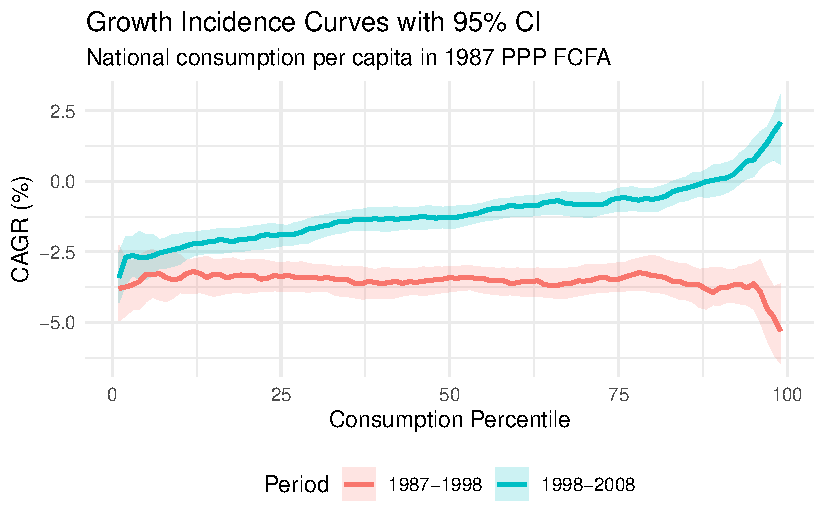
\includegraphics[keepaspectratio]{hw3_files/figure-pdf/unnamed-chunk-1-1.pdf}}

\textbf{4.e} Inequality is very likely to rise in 2008 because, between
1998 and 2008, the lowest percentiles continued to experience negative
growth while the top percentiles reached positive growth. This means
richer percentiles likely increased their consumption share while poorer
percentiles lost theirs, widening the gap between the top and bottom
percentiles.

\section{Lorenz Curves}\label{lorenz-curves}

\textbf{5.a} See Figure~\ref{fig-lorenz} for the Lorenz curves by region
and year. The x-axis and y-axis show the cumulative shares (0\% to
100\%) of the population and consumption, respectively. The dotted line
represents perfect equality, where each percentile holds an equal share
of total consumption, while curves further below it indicate greater
inequality.

\begin{figure}

\centering{

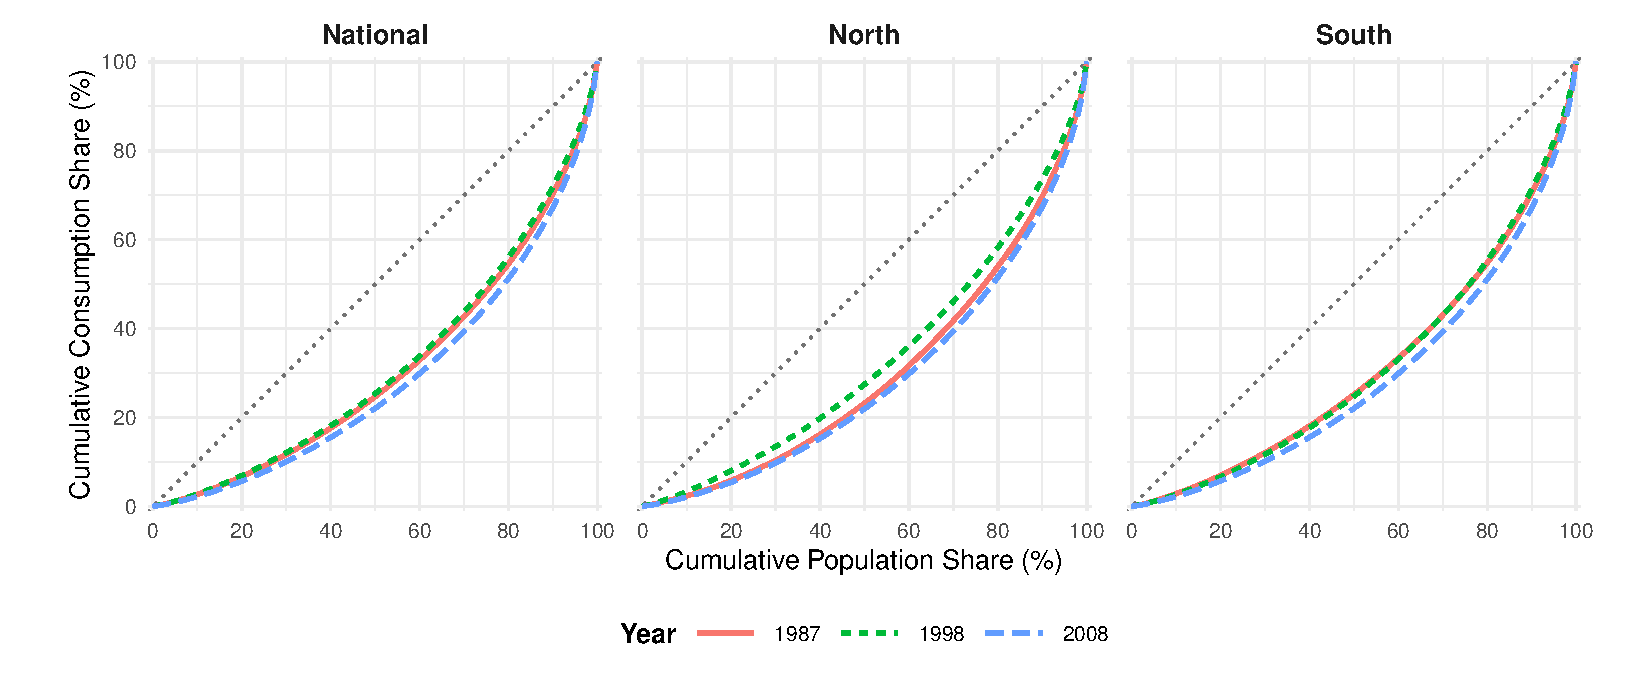
\includegraphics[width=1\linewidth,height=\textheight,keepaspectratio]{hw3_files/figure-pdf/fig-lorenz-1.pdf}

}

\caption{\label{fig-lorenz}Lorenz Curves of Daily Per Capita Consumption
by Region (1987--2008)}

\end{figure}%

\textbf{5.b} Nationally and in the North, the Lorenz curves do not
cross, while in the South the 1987 and 1998 curves cross at the 72nd
percentile. This means that in the South, low- and middle-income people
held a smaller consumption share (higher inequality) in 1998 than in
1987, while top percentiles had lower inequality. Across all regions,
the 2008 curve lies below the others, indicating inequality
unambiguously increased in 2008 relative to 1987 and 1998. Nationally,
the 1998 curve sits above the others, indicating inequality decreased in
1998, driven mostly by the North, where the 1998 curve sits well above
the others, while the South's crossing curves indicate a more complex
change.




\end{document}
